\documentclass[conference]{IEEEtran}
\IEEEoverridecommandlockouts
% The preceding line is only needed to identify funding in the first footnote. If that is unneeded, please comment it out.
\usepackage{cite}
\usepackage{pifont}
\newcommand{\cmark}{\ding{51}}
\newcommand{\xmark}{\ding{55}}
\usepackage{listings}
\usepackage{tikz}
\usepackage{enumerate}% http://ctan.org/pkg/enumerate
\usepackage{amsmath,amssymb,amsfonts}
%\usepackage{algorithmic}
\usepackage{algorithm}
\usepackage{algpseudocode}
%\usepackage[ruled,linesnumbered]
%{algorithm2e}
\usepackage{algpseudocode}
\usepackage{graphicx}
\usepackage[left=1.62cm,right=1.62cm,top=1.9cm]{geometry}
\usepackage{textcomp}
%\usepackage{hyperref}
\usepackage{xcolor}
\usepackage[table]{xcolor}
% --- Revision tags: visible [R1.x]/[R2.x] markers linking each change to a reviewer comment.
% Set \showrevtagsfalse to hide all tags (e.g., for the camera-ready version).
\newif\ifshowrevtags \showrevtagstrue
\DeclareRobustCommand{\rev}[1]{\ifshowrevtags\textcolor{red}{\textsuperscript{\textbf{[#1]}}}\fi}
\usepackage{balance}
\usepackage{algorithm}
\usepackage{algpseudocode}
\usepackage{multirow}
\usepackage{booktabs}
\usepackage{makecell}
\usepackage{balance}
\usepackage{array}
\usepackage{booktabs}
\usepackage{graphicx}
\usepackage{lscape}
\usepackage{longtable}
\usepackage{subcaption}
\setlength{\columnsep}{0.25in}
\def\BibTeX{{\rm B\kern-.05em{\sc i\kern-.025em b}\kern-.08em
    T\kern-.1667em\lower.7ex\hbox{E}\kern-.125emX}}
%\hypersetup{
 % colorlinks=true,
  %linkcolor=blue,
  %citecolor=blue,
  %urlcolor=blue
%}

\begin{document}

\title{%CONQUEST: $\mathbf{CON}$text-Aware $\mathbf{QU}$antum-Inspired Intelligence for $\mathbf{E}$spying AI-aided Cyberworm $\mathbf{S}$ecurity $\mathbf{T}$hreats in Mission Critical Systems.
CONQUEST: A Federated Context-Aware Quantum-Inspired Framework for Robust Cyberworm Detection in Mission-Critical IoT Networks
}

\author{\IEEEauthorblockN{Chimeremma Sandra Amadi, Simeon Okechukwu Ajakwe (SMIEEE)*, Ihunanya Udodiri Ajakwe,\\ Victor Ikenna Kanu, Dong-Seong Kim (SMIEEE), Taesoo Jun}
%\IEEEauthorblockA{\textit{Department of IT Convergence Engineering, Kumoh National Institute of Technology, Gumi, South Korea} \\
%$^*$Smart Computing Department, Kyungdong University, Global Campus, South Korea \\
%\textit{Kumoh National Institute of Technology} 
%Gumi, South Korea \\
%{chimesandra@yahoo.com,(simeonajlove, ihunanya.ajakwe, kanuxavier)@gmail.com, (dskim, taesoo.jun)}@kumoh.ac.kr}

 \thanks{Amadi C.S., Ajakwe I.U.,  Kanu V.I, Kim D.S., and Taesoo J. were with the Department of IT Convergence
    Engineering, Kumoh National
    Institute of Technology, Gumi, South Korea, and Ajakwe S.O. is with the Smart Computing Department, Kyungdong University, Global Campus, South Korea. e-mail: taesoo.jun@kumoh.ac.kr}
}

\maketitle

\begin{abstract}
AI-aided cyberworms capable of adaptive propagation and traffic mimicry pose severe threats to mission-critical IoT/IoV/IoD networks, rendering static intrusion detection defences ineffective. This paper proposes CONQUEST, a context-aware quantum-inspired intrusion detection framework combining seed-controlled context feature representation, variable-qubit Quantum-Inspired Particle Swarm Optimization (QPSO), and supervised LSTM(+VAE) temporal classification for cyberworm 
detection. A controlled ablation over $Q\in\{1,\dots,8\}$ \rev{R1.2}\textcolor{red}{with ten seeds shows that detection is statistically insensitive to the QPSO register size (Friedman $p{=}0.12$). With $Q{=}2$ selected on validation data, CONQUEST achieves, under leakage-free centralized evaluation on ACI-IoT, 97.11\% accuracy, 97.12\% F1-score, 0.9921 AUC, and 0.0246 MSE.}
% TODO(C10): add measured per-window latency and peak memory to the abstract. Under horizontal federated learning 
across IID, label-skew, quantity-skew, and Dirichlet regimes, CONQUEST achieves F1\,${=}$\,0.9162 and AUC\,${=}$\,0.9708 in the strongest heterogeneous setting, stabilizing at $R_{90}{=}25$ rounds with worst-client F1\,${=}$\,0.893 and $\sigma(\mathrm{F1}){=}$\,0.017, demonstrating reproducible,
\textcolor{red}{raw-data-local}, and deployment-feasible cyberworm detection for mission-critical distributed environments.
\end{abstract}

\begin{IEEEkeywords}
Cyberworm Detection, Federated Learning, Intrusion Detection System (IDS), Internet of Things (IoT), Internet of Vehicles (IoV), Internet of Drones (IoD), Mission-Critical Networks, Quantum-Inspired Particle Swarm Optimization (QPSO).  
\end{IEEEkeywords}


\section{Introduction}
\label{sec:introduction}
The rapid digitalization of mission-critical infrastructures spanning
the Internet of Things (IoT), Internet of Vehicles (IoV), and Internet
of Drones (IoD) has significantly expanded the attack surface of modern networked systems~\cite{dritsas, ajakwe2024facets}. These environments face
escalating threats from AI-aided cyberworms capable of autonomous adaptation, stealthy propagation, and mimicry of legitimate traffic, rendering static signature-based and rule-based defences progressively
ineffective~\cite{khezri}. In mission-critical settings where delayed or incorrect decisions can disrupt safety, mobility, or command operations, robust cyberworm detection is both a security requirement
and an operational necessity.
Existing IDS approaches remain limited in this context. Signature-driven methods generalize poorly to novel or polymorphic threats. Statistical
anomaly detectors suffer from high false-positive rates under noisy or heterogeneous traffic. Deep learning-based IDS improves spatio-temporal pattern recognition~\cite{al202}, yet three persistent challenges remain: (\textit{i})~optimization degrades in high-dimensional feature spaces; (\textit{ii})~performance is brittle under non-stationary data distributions; and (\textit{iii})~centralized training conflicts
with the privacy, sovereignty, and regulatory constraints prevalent in distributed mission environments.

Quantum-inspired optimization addresses the first
challenge~\cite{ajakwe2025eqai,vivekquantum}. QPSO introduces probabilistic search dynamics \textcolor{red}{that have been reported to improve exploration relative to classical metaheuristics; whether this holds for a given task must be verified against classical search under an equal evaluation budget}, yet its application to IDS remains ad- hoc, optimizer capacity is rarely analyzed systematically, stability is seldom quantified, and training-time gains are discussed without regard to deployment cost. Federated learning (FL) addresses the third challenge by keeping raw traffic local and exchanging only model updates~\cite{hamadsystematic}\textcolor{red}{; on its own, however, FL provides data locality rather than formal privacy, since model updates can still leak information through inference attacks unless secure aggregation or differential privacy is added}, yet FL-based IDS studies consistently under-report worst-client behavior, convergence stability, and robustness under realistic non-IID regimes, leaving the privacy detection reliability trade-off insufficiently characterized.

In this study, we proffer a context-aware quantum-inspired intrusion detection framework for AI-aided cyberworm detection in mission-critical networks. Here, we integrate three complementary
components: (\textit{i})~seed-controlled context-aware feature representation capturing temporal and behavioral cues relevant to
cyberworm propagation; (\textit{ii})~variable-qubit QPSO for compact, discriminative, and bounded feature selection; and
(\textit{iii})~an LSTM(+VAE) temporal classifier that captures subtle attack-state transitions. Unlike conventional IDS pipelines, this study explicitly decouples training-time feature optimization from
deployment-time inference, ensuring that runtime latency is independent of \rev{R1.1}\textcolor{red}{the QPSO register size $Q$}. This journal extension substantially advances
the conference prototype~\cite{ajakweconquest} by introducing a strong
optimized non-quantum baseline, a controlled variable-qubit ablation study over $Q\in\{1,\dots,8\}$, and a federated robustness evaluation under IID, label-skew, quantity-skew, and Dirichlet heterogeneity regimes. \textcolor{red}{Table~\ref{tab:conf_vs_journal} itemizes the methodological, experimental, and analytical differences between the two works.}

\begin{table}[!t]
\centering
\scriptsize
\caption{\textcolor{red}{Distinction between the CONQUEST conference prototype~\cite{ajakweconquest} and this journal extension.}}
\label{tab:conf_vs_journal}
\setlength{\tabcolsep}{3pt}
\renewcommand{\arraystretch}{1.10}
\color{red}
\begin{tabular}{p{1.5cm} p{2.9cm} p{3.4cm}}
\hline\toprule
\textbf{Aspect} & \textbf{Conference~\cite{ajakweconquest}} & \textbf{This journal extension} \\
\hline\toprule
\multicolumn{3}{l}{\textit{Methodological}} \\
Context features & Described qualitatively & 17 causal per-source features with explicit windows and dimensions (Table~\ref{tab:context_features}) \\
QPSO & Fixed qubit setting; selection on pooled data & Variable register size $Q$ with explicit role in initialization, rotation, and collapse (Eqs.~\eqref{eq:qpso_init}--\eqref{eq:qpso_measure}); fitted on the training split only \\
Classifier & LSTM-VAE, optimizer comparison & LSTM(+VAE) with attention, SGD, KL-regularized latent, deterministic inference \\
Training regime & Centralized only & Centralized and horizontal FL with three mask-construction modes \\
\midrule
\multicolumn{3}{l}{\textit{Experimental}} \\
Baselines & Optimizer variants & OS-CIDS, classical PSO at equal budget, context on/off $\times$ selector ablation \\
Qubit study & None & $Q\in\{1,\dots,8\}$, 10 seeds with per-seed QPSO, budget sensitivity, statistical tests \\
FL evaluation & None & IID, label-, quantity-skew, Dirichlet; FedAvg, SCAFFOLD, FLAME; $K\in\{5,10,20\}$ \\
\midrule
\multicolumn{3}{l}{\textit{Analytical}} \\
Reported metrics & DR, FPR & F1, AUC, MSE, per-class FAR/MD, selected-feature stability, per-sample latency, peak memory, $R_{90}$, $\min_k\mathrm{F1}_k$, $\sigma(\mathrm{F1})$ \\
Reproducibility & Single run & Seed-controlled, leakage-free chronological protocol, released masks \\
\hline\toprule
\end{tabular}
\end{table}

\begin{table*}[!htbp]
\centering
\scriptsize
\caption{Comparative analysis of CONQUEST against representative
related works. Limitations and gaps are specific to the
mission-critical cyberworm detection context addressed in this paper.}
\label{tab:rw_qualitative}
\setlength{\tabcolsep}{4pt}
\renewcommand{\arraystretch}{1.10}
\resizebox{\textwidth}{!}{%
\begin{tabular}{p{1.4cm} p{2.8cm} p{4.2cm} p{2.8cm} p{4.2cm}}
\hline\toprule
\textbf{Ref.} &
\textbf{Problem focus} &
\textbf{Method and key contribution} &
\textbf{Limitation} &
\textbf{Gap addressed by CONQUEST} \\
\hline\toprule

\cite{phalaagaehybrid} &
IoT IDS under resource constraints &
CNN--LSTM + attention + PSO feature selection;
strong centralized accuracy on WIoTSN &
Centralized only; no stability analysis,
reproducibility control, or FL evaluation &
Adds seed-controlled reproducibility, bounded
variable-qubit QPSO, and non-IID FL robustness
metrics ($R_{90}$, $\min_k\,\mathrm{F1}_k$,
$\sigma(\mathrm{F1})$) \\
\midrule

\cite{yuadaptive} &
IIoT IDS with class imbalance and temporal variation &
Adaptive multi-scale window segmentation +
attention transformer + adaptive focal loss;
high Acc/F1 on IIoT benchmarks &
High model complexity; centralized evaluation
only; no FL or latency/memory analysis &
Adds bounded QPSO optimization overhead
(61.2\,ms, 922\,MB) and FL deployability
analysis under heterogeneous regimes \\
\midrule

\cite{donkoloptimization} &
Communication-network IDS with optimized features &
LPPSO + ELSTM-RNN; improves detection rate
and training time on NSL-KDD and UNSW-NB15 &
Centralized benchmark only; no stochastic
stability reporting or FL evaluation &
Adds variable-capacity QPSO ablation
($Q\in\{1,\dots,8\}$) and federated robustness
under quantity-skew and Dirichlet regimes \\
\midrule

\cite{shrivashybrid} &
Network attack classification with optimized
feature subsets &
Voting ensemble + GA-PSO; improves binary
and multiclass detection accuracy &
No temporal modeling; no FL setting or
heterogeneity analysis &
Adds context-aware temporal cyberworm
modeling and non-IID federated evaluation \\
\midrule

\cite{FRIHA202217} &
Privacy-preserving IDS for agricultural IoT &
Federated DNN/CNN/RNN with server aggregation;
competitive global accuracy without raw sharing &
Trusted aggregator assumption; global metrics
only; no heterogeneity stress testing &
Adds IID, label-skew, quantity-skew, and
Dirichlet heterogeneity analysis with
worst-client and dispersion reporting \\
\midrule

\cite{herlambangfederated} &
Aggregation robustness for federated IoT IDS &
FedAvg vs.\ FedProx on IID and non-IID;
FedProx more stable under heterogeneity &
Two-client setup only; no worst-client
fairness metric or convergence stabilization
analysis &
Extends to $K{=}5$ clients across four
heterogeneity regimes; reports $R_{90}$,
$\min_k\,\mathrm{F1}_k$, and
$\sigma(\mathrm{F1})$ \\
\midrule

\cite{abdelmoniemcomprehensive} &
Heterogeneity impact on FL model quality
and fairness &
Large-scale empirical study (${\sim}$1.5K
configs); heterogeneity causes up to $4.6\times$
quality and $2.2\times$ fairness degradation &
General FL study; not IDS-specific; no
deployment or latency analysis &
Operationalizes heterogeneity findings
directly for cyberworm IDS; adds
mission-facing latency and memory bounds \\
\midrule

\cite{gefedamkd} &
Quantity-skew heterogeneity in FL &
FedAMKD adaptive mutual knowledge distillation;
outperforms FedAvg, SCAFFOLD, FedPer on
MNIST and CIFAR benchmarks &
General FL optimization study; not
IDS-specific; no deployment metrics &
Transfers quantity-skew analysis to
cyberworm IDS; adds $R_{90}$,
$\min_k\,\mathrm{F1}_k$, and
$\sigma(\mathrm{F1})$ \\
\midrule

\cite{ajakweconquest} &
Context-aware cyberworm IDS (conference
prototype) &
QPSO + LSTM-VAE on ACI-IoT; 97.5\%
detection rate, 0.8\% FPR; first
cyberworm-focused CONQUEST prototype &
Centralized only; no reproducibility
control, qubit ablation, or FL robustness
evaluation &
Journal extension adds $Q{=}1$--$8$ ablation,
\rev{R1.2}\textcolor{red}{tests it statistically}, and evaluates FL across
four heterogeneity regimes \\
\midrule

\textbf{This work} &
Mission-critical cyberworm IDS: centralized
and federated robustness &
Seed-controlled context-aware representation;
variable-qubit QPSO (\rev{R1.2}\textcolor{red}{$Q^{*}{=}2$ by validation});
supervised LSTM(+VAE)+SGD; HFL under IID,
label-skew, quantity-skew, Dirichlet &
Additional training-time overhead from
QPSO optimization &
Uniquely integrates (i)~reproducibility,
(ii)~bounded QPSO with capacity ablation,
(iii)~non-IID FL robustness, and
(iv)~mission-facing deployability metrics
in a single unified framework \\

\hline\toprule
\end{tabular}}
\end{table*}


%The key contributions are as follows:
%\begin{itemize}
    %\item We propose CONQUEST, a reproducible context-aware quantum-inspired IDS framework for robust detection of AI-aided cyberworms in mission-critical IoT/IoV/IoD environments.
    %\item We establish, through a controlled variable-qubit ablation, that QPSO-based feature selection exhibits an expressiveness stability trade-off with a stability-optimal operating point at $Q{=}6$, yielding 96.85\% accuracy and F1-score, 0.9947 AUC, and 0.0240 MSE under centralized evaluation on the ACI-IoT dataset, with end-to-end latency of 61.2\,ms and memory of 922\,MB.

    %\item We evaluate CONQUEST under horizontal federated learning across four heterogeneity regimes, quantifying deployability via worst-client reliability ($\min_k\,\mathrm{F1}_k{=}0.893$), inter-client dispersion ($\sigma(\mathrm{F1}){=}0.017$), and convergence stability ($R_{90}{=}25$), demonstrating a centralised to federated performance gap of only 2.9\% in F1-score.
%\end{itemize}

\subsection{Key Contributions}
The core contributions of this manuscript, which significantly advance the preliminary conference prototype \cite{ajakweconquest}, are as follows:

\begin{itemize}
    \item \textbf{Framework Reproducibility and Contextual Synergy:} We propose \textit{CONQUEST}, a high-fidelity, seed-controlled IDS framework that uniquely harmonizes context-aware feature engineering with quantum-inspired optimization. By enforcing a global deterministic protocol, governing both Stage $\mathcal{Q}_{Q}$ mask sampling and Stage D neural weight initialization, \textcolor{red}{and by re-executing QPSO for every seed so that reported variance includes the optimizer's own stochasticity, we make the run-to-run variability of quantum-inspired selection explicit and measurable.}

    \item \textbf{\rev{R1.1, R1.2}\textcolor{red}{Characterization of the Qubit-Register Size}:} Through an extensive variable-qubit ablation study ($Q \in \{1, \dots, 8\}$), we characterize the expressiveness-stability trade-off in QPSO-based feature selection. \textcolor{red}{We make explicit how $Q$ enters the search, show that it interpolates between near-random exploration (small $Q$) and frozen exploitation (large $Q$), and show, with Friedman and Holm-corrected Wilcoxon tests over ten seeds and a search-budget sensitivity analysis, that detection is statistically insensitive to $Q$ within the tested range, so the operating point $Q^{*}{=}2$ is fixed by a pre-declared validation rule.}

    \item \textbf{Stress-Testing Federated Robustness under Heterogeneity:} We provide the first systematic evaluation of quantum-inspired IDS under four distinct federated heterogeneity regimes: IID, label-skew, quantity-skew, and Dirichlet partitions. By introducing mission-centric metrics—specifically thresholded stabilization ($R_{90}=25$), worst-client reliability ($\min_{k} F1_{k}=0.893$), and inter-client dispersion ($\sigma(F1)=0.017$), we demonstrate that \textit{CONQUEST} bounds the centralized-to-federated performance gap to a marginal 2.9\%. \textcolor{red}{We further vary the number of clients ($K\in\{5,10,20\}$) and compare three privacy-compatible mask-construction modes for non-IID clients.}

    \item \textbf{Ablative Attribution via Optimized Baseline:} We introduce a rigorous non-quantum baseline (\textit{OS-CIDS}) \textcolor{red}{and a factorial ablation (context features on/off $\times$ variance vs.\ QPSO selection), together with a classical PSO baseline at an equal fitness-evaluation budget, to separate the contributions of context-aware representation and quantum-inspired search.}
\end{itemize}

The remainder of this paper is organized as follows.
Section~\ref{sec:related_works} reviews related work.
Section~\ref{sec:conquest_overview} presents the CONQUEST architecture and methodology. Section~\ref{sec:results_discussion} reports
experimental results. Section~\ref{sec:conclusion} concludes with future directions.




\section{\textbf{related works}}
\label{sec:related_works}

Effective cyberworm detection in mission-critical networks demands
solutions that jointly address high-dimensional traffic complexity,
privacy-constrained distributed deployment, and operational
robustness under heterogeneous conditions. Prior work has advanced
each of these dimensions independently, yet their integrated
treatment under a single deployment-oriented framework remains
absent. This section traces that progression to motivate the design
of CONQUEST.

\subsection{Deep Temporal Intrusion Detection}

Intrusion detection in IoT/IIoT environments has shifted from
signature-driven and shallow-learning approaches toward deep
architectures that model temporal traffic behavior directly,
reflecting the reality that cyberworm propagation manifests as
low-intensity, time-evolving deviations rather than abrupt
anomalies. CNN--LSTM and attention-based variants improve temporal
discrimination by combining local feature extraction with long-range
dependency modeling~\cite{phalaagaehybrid,yuadaptive}, while
lightweight recurrent autoencoding detectors reduce inference cost
without sacrificing real-time sensitivity~\cite{yupgtad}. Multi-view
flow packet pipelines further reduce single-view detection
errors~\cite{sudyanaflow}. These works confirm that temporal deep
modeling is necessary for complex traffic, yet they share a common
limitation: all operate on the full, high-dimensional feature space
without principled selection, increasing both computational burden
and sensitivity to noisy or irrelevant features. This raises a
practical question, how to identify compact, discriminative feature
subsets that preserve temporal structure while reducing optimization
cost which brings feature selection to the center of the design
problem.

\subsection{Feature Selection via Swarm and Quantum-Inspired Optimization}

Recognizing that intrusion telemetry is typically high-dimensional
and redundant, a substantial body of work formulates feature
selection as a combinatorial optimization problem and applies swarm
or evolutionary search. PSO-coupled temporal backbones reduce
dimensionality while preserving discriminative
structure~\cite{donkoloptimization}. Multi-objective formulations
balance detection performance against subset
size~\cite{sezginmulti,raeisientropy}, metaheuristics optimize model
hyperparameters directly~\cite{kishoreimproved}, and ensemble wrapper
methods extend this line to fog and cloud anomaly
detection~\cite{yaseenefficient,bilalevaluation,maryenhancing,shrivashybrid}.
Quantum-inspired sampling has recently been introduced as a stronger
exploration mechanism~\cite{vivekquantum}, yet it is consistently
treated as a drop-in improvement without controlled analysis of how
optimizer expressiveness affects convergence stability, overhead, or
deployment-time cost. Crucially, these studies report only final
detection performance with limited analysis of stochastic stability
or latency and memory behavior properties that are non-negotiable
in mission-critical deployment. More fundamentally, all of these
systems assume centralized access to training data, an assumption
that is increasingly violated in distributed mission environments
where raw traffic cannot leave each node due to sovereignty and
regulatory constraints. Addressing this constraint requires moving
from centralized optimization to privacy-preserving distributed
training, which is precisely what federated learning provides.

\subsection{Federated Learning for Distributed IDS}

Federated learning (FL) has emerged as the dominant paradigm for
privacy-preserving collaborative intrusion detection, keeping raw
traffic local and exchanging only model updates~\cite{hamadsystematic}.
Representative FL-IDS systems span agricultural IoT
deployments~\cite{FRIHA202217}, privacy-preserving distributed
designs~\cite{amrosecuring}, federated sequential
detectors~\cite{selvamfederated,anweradvanced}, and unsupervised
VAE/GMM anomaly detectors targeting unknown-threat
coverage~\cite{camposfederated}. FedProx has been shown to outperform
FedAvg under non-IID partitions on CICIoT2023~\cite{herlambangfederated},
secure aggregation strengthens FL against collusion and replay
attacks~\cite{yaoenhanced}, and fog-hierarchical architectures improve
scalability across distributed sites~\cite{alsalehheterogeneity,islamprivacy}.
These works confirm that FL can achieve competitive detection accuracy
without raw data sharing. However, they consistently evaluate only
global average metrics under IID or mildly non-IID settings, masking
the behavior of underperforming clients and obscuring whether the
system is genuinely robust or merely average-robust. In mission
deployments, where a single compromised subsystem can propagate a
worm across the network, tail performance matters as much as mean
performance, a distinction that existing FL-IDS work does not
address. This motivates a closer look at heterogeneity modeling and
its effect on worst-case detection reliability.

\subsection{Federated Robustness Under Heterogeneous Data}

Motivated by the inadequacy of IID assumptions, a dedicated line of
work studies FL robustness under realistic heterogeneity. Large-scale
empirical analyses confirm that device and behavioral heterogeneity
substantially degrades model quality and fairness, with up to
$4.6\times$ quality reduction and $2.2\times$ fairness degradation
reported across heterogeneous
configurations~\cite{abdelmoniemcomprehensive}, establishing that
heterogeneity must be a primary design variable, not a benchmark
afterthought. Hierarchical Dirichlet partitioning extends label-skew
simulation with feature-space
clustering~\cite{arisdakessiantwo}, quantity-skewed non-IID learning
has been addressed through adaptive mutual knowledge
distillation~\cite{gefedamkd} and regularization-adjusted gradient
optimization~\cite{chaaddressing}, and within the IDS domain,
adaptive personalized FL improves per-client
utility~\cite{almansouradaptive} while stability-aware client
selection reduces convergence
instability~\cite{vinothinienhancing}. Despite these advances, no
existing work connects non-IID robustness to mission-facing IDS
criteria: none report thresholded stabilization ($R_{90}$),
worst-client detection utility ($\min_k\,\mathrm{F1}_k$), or
deployment readiness under operational traffic-volume imbalance.
More broadly, the literature has yet to combine temporal deep
modeling, capacity-controlled quantum-inspired feature selection,
and federated heterogeneity robustness within a single reproducible
pipeline; the precise integration that CONQUEST provides.

\subsection{Research Gap and Positioning of CONQUEST}

Table~\ref{tab:rw_qualitative} positions CONQUEST relative to
representative recent work. The foregoing review identifies a clear
and consistent gap: while temporal IDS, swarm-based feature
selection, and federated learning have each advanced significantly,
no existing work integrates all three under a unified,
deployment-oriented methodology. Specifically, no prior system
simultaneously provides seed-controlled reproducibility, context-aware
temporal feature construction for cyberworm dynamics,
capacity-controlled quantum-inspired selection with bounded latency
and memory, and federated robustness reporting under mission-relevant
quantity-skew. The conference prototype of
CONQUEST~\cite{ajakweconquest} established the feasibility of
QPSO-based feature selection with a temporal backbone for centralized
cyberworm detection; the present journal extension closes the
remaining gaps by adding a controlled variable-qubit ablation over
$Q\in\{1,\dots,8\}$, a strong optimized non-quantum baseline for
rigorous comparison, and a comprehensive federated evaluation across
IID, label-skew, quantity-skew, and Dirichlet regimes quantified
through $R_{90}$, $\min_k\,\mathrm{F1}_k$, and $\sigma(\mathrm{F1})$.





\section{\textbf{system overview and design objectives}}
\label{sec:conquest_overview}

CONQUEST is a latency-constrained, seed-controlled intrusion
detection framework engineered for mission-critical IoT/IoV/IoD
networks subject to real-time execution, bounded memory, and data
sovereignty constraints. Given identical data partitions,
hyperparameters, and a fixed random seed, the pipeline produces
identical outputs; QPSO ablation results are therefore reported as
mean$\pm$std over repeated seed-controlled runs to account for
stochastic mask sampling. Table~\ref{tab:acronyms_notations}
lists non-standard acronyms and symbols. Fig.~\ref{fig:conquest_architecture}
illustrates the end-to-end architecture.

\begin{table}[!t]
\centering
\scriptsize
\caption{Non-Standard Acronyms, Symbols, and Notations}
\label{tab:acronyms_notations}
\setlength{\tabcolsep}{4pt}
\renewcommand{\arraystretch}{1.05}
\begin{tabular}{p{1.8cm} p{5.2cm}}
\hline\toprule
\textbf{Notation / Acronym} & \textbf{Description} \\
\hline\toprule
CONQUEST  & CONtext-Aware QUantum-Inspired Intelligence
            framework for cyberworm detection \\
QPSO      & Quantum-Inspired Particle Swarm Optimization \\
QCIDS     & Quantum-Context Intrusion Detection System \\
S-CIDS    & Static Centralized IDS (conference baseline) \\
OS-CIDS   & Optimized Static Centralized IDS \\
HFL       & Horizontal Federated Learning \\
FedAvg    & Federated Averaging \\
\midrule
$Q$                     & \rev{R1.1}\textcolor{red}{Qubit-register size; sets the
                          QPSO amplitude initialization, rotation-angle
                          bound, and collapse probability
                          (Eqs.~\eqref{eq:qpso_init}--\eqref{eq:qpso_collapse})} \\
\rev{R1.1}\textcolor{red}{$d$, $k$} & \textcolor{red}{Number of input features; number
                          of selected features ($k=\|\mathbf{m}\|_0$)} \\
\rev{R1.1}\textcolor{red}{$P$, $I$} & \textcolor{red}{QPSO particles; QPSO iterations} \\
$K$                     & Number of federated clients \\
$\alpha$                & Dirichlet concentration parameter \\
$\theta$                & Model parameter vector \\
$\mathcal{D}_k$         & Local dataset of client $k$ \\
$\mathbf{m}^{*}$        & Optimal fixed feature mask
                          at deployment \\
$\mathcal{L}_{\rm e2e}$ & End-to-end pipeline latency \\
$\mathcal{M}(Q)$        & Memory usage at qubit setting $Q$ \\
$R_{90}$                & Round at which global F1 reaches
                          90\% of terminal F1 \\
$\min_k\,{\rm F1}_k$    & Worst-client F1 score \\
$\sigma({\rm F1})$      & Inter-client F1 dispersion \\
\hline\toprule
\end{tabular}
\end{table}

Let $\mathbf{X}=\{x_t\}_{t=1}^{T}$ denote raw network traffic
observations. CONQUEST applies a three-stage transformation:
\begin{equation}
\mathbf{X} \xrightarrow{\mathcal{C}} \mathbf{Z}
           \xrightarrow{\mathcal{Q}_{Q}} \mathbf{Z}^{*}
           \xrightarrow{\mathcal{D}} \hat{y},
\label{eq:pipeline}
\end{equation}
where $\mathcal{C}$ is context-aware feature conditioning
(Section~\ref{subsec:feature_pipeline}), $\mathcal{Q}_{Q}$ is
variable-qubit quantum-inspired feature selection
(Section~\ref{subsec:qpsomethod}), and $\mathcal{D}$ is temporal
binary classification (Section~\ref{subsec:model_training}).
\rev{R1.1}\textcolor{red}{The register size $Q$ does not change the
dimension of a particle, which is always $d$; it controls the
exploration--exploitation balance of the search
(Section~\ref{subsec:qpsomethod}). CONQUEST selects $Q$
empirically on validation data.} Quantum-inspired computation is strictly
confined to $\mathcal{Q}_{Q}$ during training. At deployment, only
$\mathcal{C}$ and $\mathcal{D}$ execute using the fixed stored mask
$\mathbf{m}^{*}$, ensuring inference latency independent of $Q$:
\begin{equation}
\mathcal{L}_{\text{infer}}(Q) =
\mathcal{L}_{\text{infer}}^{\text{classical}}.
\label{eq:infer_invariance}
\end{equation}
Training executes under centralized or federated regimes. In
federated mode, $K$ clients with heterogeneous local datasets
$\{\mathcal{D}_k\}_{k=1}^{K}$ train collaboratively via FedAvg:
\begin{equation}
\theta^{(r+1)} = \sum_{k=1}^{K}
\frac{|\mathcal{D}_k|}{\sum_{j=1}^{K}|\mathcal{D}_j|}
\,\theta_k^{(r+1)},
\label{eq:fedavg_overview}
\end{equation}
exchanging only model updates to preserve data sovereignty.
CONQUEST is designed to jointly satisfy $\mathcal{L}_{\rm infer}
\leq \mathcal{L}_{\max}$, $\mathcal{M}(Q)\leq 1$\,GB, bounded
$\sigma(\mathrm{F1})$ under non-IID heterogeneity, and
deployability under both execution regimes.

\begin{figure*}[!htbp]
    \centering
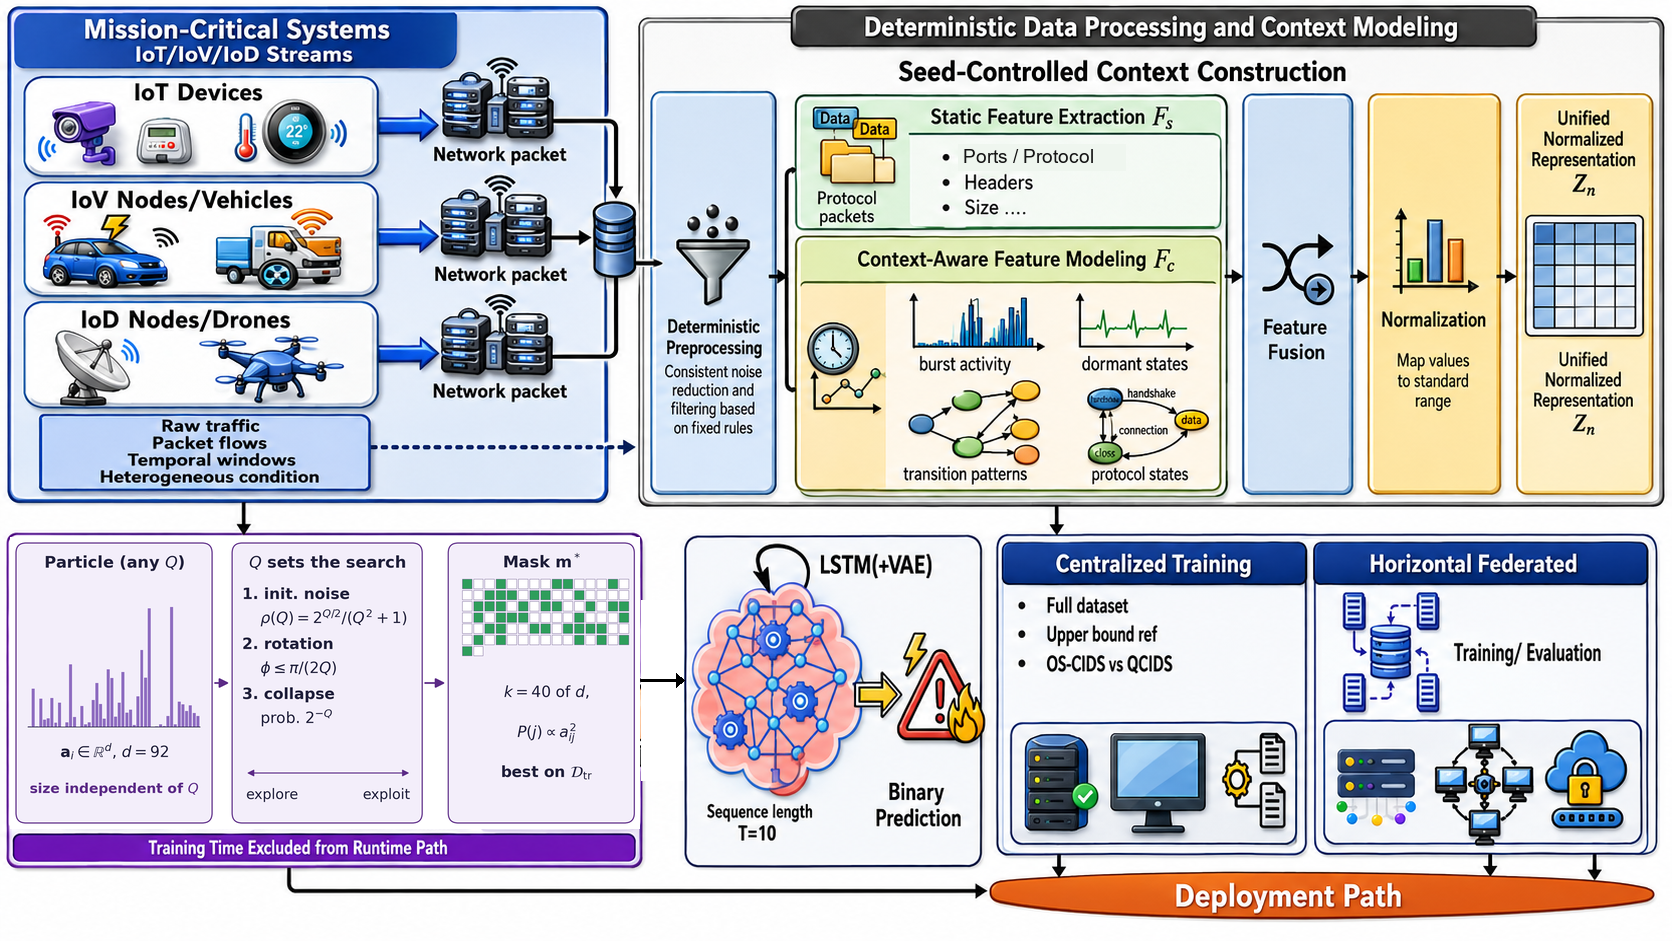
\includegraphics[width=0.8\linewidth]{images/CON-PICTURE2_rev.png}
    \caption{CONQUEST End-to-end architecture illustrating the three-stage transformation $\mathbf{X} \xrightarrow{\mathcal{C}} \mathbf{Z} \xrightarrow{\mathcal{Q}_{Q}} \mathbf{Z}^{*} \xrightarrow{\mathcal{D}} \hat{y}$, where Stage $\mathcal{C}$ (CAP module) fuses static descriptors $\mathbf{F}_s$ and offline context-aware features $\mathbf{F}_c$ into normalized representation $\mathbf{Z}_n$, Stage $\mathcal{Q}_{Q}$ applies variable-qubit QPSO \rev{R1.1}\textcolor{red}{to $d$-dimensional amplitude particles whose initialization, rotation, and collapse are set by $Q$ (Algorithm~\ref{alg:qpso}), and returns the best-scoring $k$-feature mask $\mathbf{m}^{*}$ found on $\mathcal{D}_{\rm tr}$, with $Q$ chosen on $\mathcal{D}_{\rm va}$}, and Stage $\mathcal{D}$ executes supervised LSTM(+VAE)+SGD binary classification under centralized or horizontal federated training.}
\label{fig:conquest_architecture}
\end{figure*}


%% ----------------------------------------------------------
\subsection{Data Processing and Context-Aware Feature
            Representation (Stage~$\mathcal{C}$)}
\label{subsec:feature_pipeline}
%% ----------------------------------------------------------

Raw traffic $\mathbf{X}(t)\in\mathbb{R}^{N\times d}$ is
transformed into a unified feature representation via a
seed-controlled deterministic preprocessing pipeline:
\begin{equation}
\mathbf{X}(t) \xrightarrow{\mathcal{P}}
\mathbf{F}_s \oplus \mathbf{F}_c = \mathbf{Z},
\label{eq:feature_fusion}
\end{equation}
where $\mathbf{F}_s$ denotes static flow descriptors
(\textcolor{red}{ports, protocol, flow duration, packet and byte
counts, packet-length statistics, inter-arrival times, flag
counts, and bulk and activity statistics produced by
CICFlowMeter, $|\mathbf{F}_s|=75$; flow identifiers, IP
addresses, and timestamps are excluded from the feature vector to
prevent identity shortcuts, and so are the four \texttt{Idle}
fields, which in ACI-IoT store absolute epoch timestamps and would
leak capture time}) and $\mathbf{F}_c$ encodes
context-aware features computed offline via fixed sliding-window operators and transition statistics. To ensure end-to-end reproducibility, this global fixed seed governs both the probabilistic \textcolor{red}{measurement} sampling in Stage $\mathcal{Q}_{Q}$ and the stochastic weight initialization of the Stage D temporal classifier. Context features capture burst
activity, dormant intervals, and protocol state transitions that
are not separable under static feature selection alone; no live
behavioral monitoring is performed at runtime.

\textcolor{red}{Table~\ref{tab:context_features} defines the
$|\mathbf{F}_c|=17$ context features. Flows are sorted by
timestamp and grouped by source IP, which serves only as a
grouping key. Every feature is causal: it is computed from the
source's earlier flows (excluding the current flow),
using window lengths $W\in\{10,60\}$\,s. Ties at the 1\,s
timestamp resolution are broken by capture order. Context
features are computed on the full chronological stream before
subsampling, so that window statistics reflect real traffic
density.}

\begin{table}[!t]
\centering
\scriptsize
\caption{\textcolor{red}{Context-aware features $\mathbf{F}_c$. All
features are causal and grouped by source IP; $W$ is the
look-back window.}}
\label{tab:context_features}
\setlength{\tabcolsep}{3pt}
\renewcommand{\arraystretch}{1.08}
\color{red}
\begin{tabular}{p{1.3cm} p{2.6cm} p{2.5cm} c}
\hline\toprule
\textbf{Group} & \textbf{Feature} & \textbf{Window} & \textbf{Dim.} \\
\hline\toprule
Burst & Flow count from source & $W\in\{10,60\}$\,s & 2 \\
      & Packet rate (fwd+bwd pkts$/W$) & $W\in\{10,60\}$\,s & 2 \\
      & Byte rate (fwd+bwd bytes$/W$) & $W\in\{10,60\}$\,s & 2 \\
\midrule
Dormant interval & Time since source's previous flow & -- & 1 \\
      & Log of the above & -- & 1 \\
      & Largest inter-flow gap & 60\,s & 1 \\
\midrule
Sliding-window diversity & Distinct destination IPs & $W\in\{10,60\}$\,s & 2 \\
      & Distinct destination ports & $W\in\{10,60\}$\,s & 2 \\
\midrule
Transition & Protocol switch vs.\ previous flow (0/1) & -- & 1 \\
      & Number of protocol switches & 60\,s & 1 \\
      & Fraction of flows with SYN set & 60\,s & 1 \\
      & Destination-port switch vs.\ previous flow (0/1) & -- & 1 \\
\midrule
\multicolumn{3}{l}{\textbf{Total}} & \textbf{17} \\
\hline\toprule
\end{tabular}
\end{table}

\textcolor{red}{The fused representation has $d=92$ features.
A class-balanced subsample of 80{,}000 flows (40{,}000 benign,
40{,}000 attack; attack-type proportions preserved) is drawn with
a fixed seed and re-sorted chronologically. ACI-IoT attacks are
clustered in time, so a purely chronological 70/15/15 split would
leave $\mathcal{D}_{\rm te}$ entirely benign. We therefore use a
blocked temporal split: the chronological stream is cut into
contiguous 500-flow blocks, the blocks are assigned to
$\mathcal{D}_{\rm tr}$, $\mathcal{D}_{\rm va}$, and
$\mathcal{D}_{\rm te}$ (70/15/15) by a seeded shuffle, and the
first $T=10$ flows of every block are purged. Sliding windows of
length $T=10$ are built only within a block, so no window spans
two splits and no flow appears in two windows of different
splits. The resulting splits contain 54{,}890 / 11{,}760 /
11{,}760 flows with attack fractions of 47.5\% / 53.6\% /
58.2\%; $\mathcal{D}_{\rm tr}$ covers all ten attack types,
$\mathcal{D}_{\rm va}$ seven, and $\mathcal{D}_{\rm te}$ six.}
The fused
representation is normalized as
\begin{equation}
\mathbf{Z}_n = \mathcal{N}(\mathbf{Z}),\quad
\mathbf{Z}_n \in [0,1]^d,
\label{eq:normalization}
\end{equation}
using parameters computed on $\mathcal{D}_{\rm tr}$ and applied
without update to $\mathcal{D}_{\rm va}$ and $\mathcal{D}_{\rm te}$
\textcolor{red}{(values outside $[0,1]$ are clipped)},
eliminating feature-induced confounding across centralized and
federated regimes. The resulting $\mathbf{Z}_n$ is the fixed input
to Stage~$\mathcal{Q}_{Q}$. Fig.~\ref{fig:pipeline} illustrates
the preprocessing and context-feature construction pipeline.

%% ----------------------------------------------------------
\subsection{Variable-Qubit QPSO Feature Selection
            (Stage~$\mathcal{Q}_{Q}$)}
\label{subsec:qpsomethod}
%% ----------------------------------------------------------

Stage $\mathcal{Q}_{Q}$ learns a sparse binary feature mask
$\mathbf{m}\in\{0,1\}^d$ that gates the normalized input:
\begin{equation}
\tilde{\mathbf{z}} = \mathbf{m}\odot\mathbf{z}_n,\quad
\|\mathbf{m}\|_0 = k \ll d,
\label{eq:mask_gate}
\end{equation}
where $\odot$ denotes element-wise multiplication.
\rev{R1.1}\textcolor{red}{Each of the $P$ particles $i$ holds a non-negative
amplitude vector $\mathbf{a}_i\in\mathbb{R}_{\ge 0}^{d}$ with
$\sum_j a_{i,j}=1$, one amplitude per feature; the particle
dimension is $d$ for every $Q$. The register size $Q$ enters the
search at three points. First, amplitudes are initialized at the
uniform amplitude of a $Q$-qubit register plus Gaussian noise; after
normalization only the relative perturbation
$\rho(Q)=2^{Q/2}/(Q^{2}+1)$ matters (Table~\ref{tab:q_constants}):}
\begin{equation}
\textcolor{red}{a_{i,j}^{(0)} \propto \Bigl|\,2^{-Q/2} +
\tfrac{\xi_{i,j}}{Q^{2}+1}\Bigr|,\quad
\xi_{i,j}\sim\mathcal{N}(0,1).}
\label{eq:qpso_init}
\end{equation}
\rev{R1.1}\textcolor{red}{Second, at iteration $t$ each particle is rotated
toward its personal-best amplitude $\mathbf{a}_i^{\rm pb}$ and the
global-best amplitude $\mathbf{a}^{\rm gb}$ by an angle whose
upper bound decreases with $Q$:}
\begin{align}
\textcolor{red}{\phi_t} &\textcolor{red}{= \frac{\pi}{2Q}\Bigl(1-\frac{t}{I}\Bigr),}
\label{eq:qpso_angle}\\
\textcolor{red}{\mathbf{a}_i} &\textcolor{red}{\leftarrow \mathbf{a}_i
+ r_1\cos\phi_t\,(\mathbf{a}_i^{\rm pb}-\mathbf{a}_i)
+ r_2\sin\phi_t\,(\mathbf{a}^{\rm gb}-\mathbf{a}_i),}
\label{eq:qpso_rotation}
\end{align}
\rev{R1.1}\textcolor{red}{with $r_1,r_2\sim\mathcal{U}(0,1)$ drawn per
particle and iteration. Third, each amplitude independently
``collapses'' to a fresh random value with a probability that
decays exponentially in $Q$, after which the vector is
renormalized:}
\begin{equation}
\textcolor{red}{a_{i,j} \leftarrow u_{i,j}\sim\mathcal{U}(0,1)
\ \text{ with prob. } 2^{-Q},\qquad
\mathbf{a}_i \leftarrow |\mathbf{a}_i| / \|\mathbf{a}_i\|_1 .}
\label{eq:qpso_collapse}
\end{equation}
\rev{R1.1}\textcolor{red}{A mask is obtained by measurement: $k$ distinct
feature indices are drawn without replacement with probabilities
$\pi_{i,j}=a_{i,j}^{2}/\sum_{l}a_{i,l}^{2}$, and $m_{i,j}=1$ for
the drawn indices,}
\begin{equation}
\textcolor{red}{\mathbf{m}_i = \textsc{Measure}_k(\boldsymbol{\pi}_i),
\qquad \|\mathbf{m}_i\|_0 = k .}
\label{eq:qpso_measure}
\end{equation}
\rev{R1.1}\textcolor{red}{The deployed mask $\mathbf{m}^{*}$ is the
highest-fitness mask measured during the search, i.e.\ the
measurement that produced the final global best, as in standard
PSO. Hence $k$ is a fixed design parameter ($k=40$ in all
experiments), and $Q$ shapes \emph{which} $k$ features are found,
not how many. Algorithm~\ref{alg:qpso} summarizes the procedure and
Table~\ref{tab:q_constants} lists the constants set by each $Q$.}

\begin{algorithm}[!t]
\caption{\rev{R1.1}\textcolor{red}{Variable-qubit QPSO feature selection
(Stage~$\mathcal{Q}_{Q}$). Lines marked $\triangleright Q$ are the only
places where $Q$ enters.}}
\label{alg:qpso}
\color{red}
\small
\begin{algorithmic}[1]
\Require $\mathbf{Z}_{\rm tr}\in[0,1]^{N\times d}$, labels $\mathbf{y}_{\rm tr}$, register size $Q$, particles $P$, iterations $I$, subset size $k$
\Ensure Mask $\mathbf{m}^{*}\in\{0,1\}^{d}$ with $\|\mathbf{m}^{*}\|_0=k$
\For{$i=1$ to $P$}
  \State $\mathbf{a}_i\gets$ Eq.~\eqref{eq:qpso_init}, normalized \Comment{$\triangleright Q$}
  \State $\mathbf{m}_i\gets\textsc{Measure}_k(\mathbf{a}_i)$; $J_i\gets\mathcal{J}(\mathbf{m}_i)$ on $\mathcal{D}_{\rm tr}$
  \State $\mathbf{a}_i^{\rm pb}\gets\mathbf{a}_i$; $J_i^{\rm pb}\gets J_i$
\EndFor
\State $i^{\star}\gets\arg\max_i J_i$; $\mathbf{a}^{\rm gb}\gets\mathbf{a}_{i^{\star}}$; $\mathbf{m}^{*}\gets\mathbf{m}_{i^{\star}}$; $J^{*}\gets J_{i^{\star}}$
\For{$t=0$ to $I-1$}
  \State $\phi_t\gets\frac{\pi}{2Q}(1-t/I)$ \Comment{$\triangleright Q$}
  \For{$i=1$ to $P$}
    \State $\mathbf{a}_i\gets$ rotation toward $\mathbf{a}_i^{\rm pb},\mathbf{a}^{\rm gb}$, Eq.~\eqref{eq:qpso_rotation}
    \State reset each $a_{i,j}$ w.p.\ $2^{-Q}$; normalize, Eq.~\eqref{eq:qpso_collapse} \Comment{$\triangleright Q$}
    \State $\mathbf{m}_i\gets\textsc{Measure}_k(\mathbf{a}_i)$, Eq.~\eqref{eq:qpso_measure}; $J_i\gets\mathcal{J}(\mathbf{m}_i)$
    \If{$J_i>J_i^{\rm pb}$}
      \State $\mathbf{a}_i^{\rm pb}\gets\mathbf{a}_i$; $J_i^{\rm pb}\gets J_i$
    \EndIf
    \If{$J_i>J^{*}$}
      \State $\mathbf{a}^{\rm gb}\gets\mathbf{a}_i$; $\mathbf{m}^{*}\gets\mathbf{m}_i$; $J^{*}\gets J_i$
    \EndIf
  \EndFor
\EndFor
\State \Return $\mathbf{m}^{*}$ \Comment{$P(I+1)$ fitness evaluations}
\end{algorithmic}
\end{algorithm}

\begin{table}[!t]
\centering
\scriptsize
\caption{\rev{R1.1}\textcolor{red}{Search constants set by the register size
$Q$ ($d=92$). $\rho$: relative initial perturbation; $\phi_{\max}$:
rotation-angle bound; $2^{-Q}$: per-amplitude collapse probability;
$d\,2^{-Q}$: expected resets per particle and iteration.}}
\label{tab:q_constants}
\setlength{\tabcolsep}{5pt}
\renewcommand{\arraystretch}{1.05}
\color{red}
\begin{tabular}{cccccc}
\hline\toprule
$Q$ & $\rho(Q)$ & $\phi_{\max}$ (deg) & $2^{-Q}$ & $d\,2^{-Q}$ & Regime \\
\hline\toprule
1  & 0.71 & 90.0 & 0.500  & 46.0 & near-random \\
2  & 0.40 & 45.0 & 0.250  & 23.0 & exploratory \\
3  & 0.28 & 30.0 & 0.125  & 11.5 & exploratory \\
4  & 0.24 & 22.5 & 0.063  & 5.75 & balanced \\
5  & 0.22 & 18.0 & 0.031  & 2.88 & balanced \\
6  & 0.22 & 15.0 & 0.016  & 1.44 & balanced \\
7  & 0.23 & 12.9 & 0.008  & 0.72 & exploitative \\
8  & 0.25 & 11.3 & 0.004  & 0.36 & exploitative \\
9  & 0.29 & 10.0 & 0.002  & 0.18 & near-frozen \\
10 & 0.32 & 9.0  & 0.001  & 0.09 & near-frozen \\
\hline\toprule
\end{tabular}
\end{table}

\rev{R1.1, R1.2}\textcolor{red}{\textit{Interpretation of $Q$.} For $Q=1$, the
rotation bound is $\pi/2$ and half of all amplitudes are reset at
every iteration, so the search is close to random sampling. As
$Q$ increases, the bound shrinks to $\pi/16$ at $Q=8$, the update
is dominated by the personal-best term ($\cos\phi_t\to 1$), and
the expected number of resets per particle and iteration,
$d\,2^{-Q}$, falls below one. $Q$ therefore interpolates between
exploration and exploitation, with a risk of premature convergence
at large $Q$ under a finite budget. Beyond $Q=8$ the collapse
probability is at most $0.2\%$ and the global-best pull
($\sin\phi_t<0.2$) is weak, so the search is effectively frozen
around its initialization; this motivates the tested range
$Q\in\{1,\dots,8\}$. The range is extended to $Q=10$ in the
budget-sensitivity analysis to confirm this.}

\rev{R1.1}\textcolor{red}{We stress that CONQUEST is quantum-\emph{inspired}
and runs on classical hardware: no $2^{Q}$-dimensional state vector
is simulated, and the particle dimension is $d$ for every $Q$. The
term ``qubit'' refers to the register whose uniform amplitude
$2^{-Q/2}$ and measurement-collapse probability $2^{-Q}$ motivate
the three $Q$-dependent constants above; $Q$ is therefore a single
interpretable hyperparameter that sets the exploration schedule of
the swarm, not a measure of model capacity.}

\rev{R1.1}\textcolor{red}{\textit{Empirical search dynamics.}
Fig.~\ref{fig:qpso_dynamics} verifies this interpretation by
running Algorithm~\ref{alg:qpso} on $\mathcal{D}_{\rm tr}$ for
$Q\in\{1,\dots,10\}$ and ten seeds, without training any
classifier. Three regimes appear. For $Q=1$, the amplitude entropy
drops only to $0.75$ and stays there, because about half of all
amplitudes are reset at every iteration; the swarm keeps sampling
almost uniformly. For $Q\in\{4,\dots,7\}$, entropy falls to
$0.26$--$0.34$ within a few iterations, and swarm diversity dips
most strongly for $Q\in\{3,\dots,6\}$, i.e.\ the search
concentrates on a feature subset.
For $Q\ge 9$, entropy decreases slowly and remains near $0.5$--$0.6$,
because the small rotation angle and rare collapses barely move the
particles from their initialization. The best Fisher fitness found
follows the same pattern: it is highest at intermediate $Q$
($5034\pm374$ at $Q=5$) and lowest at the extremes
($4544\pm344$ at $Q=1$, $4574\pm304$ at $Q=10$). Returning the
best evaluated mask matters most in the exploitative regime: a
fresh measurement of the final global-best amplitude retains $98\%$
of the best fitness at $Q=1$ but only $45\%$ at $Q=10$, because the
amplitudes at large $Q$ stay close to their spread-out
initialization, so re-sampling them rarely reproduces the best
subset.}

\begin{figure*}[!t]
\centering
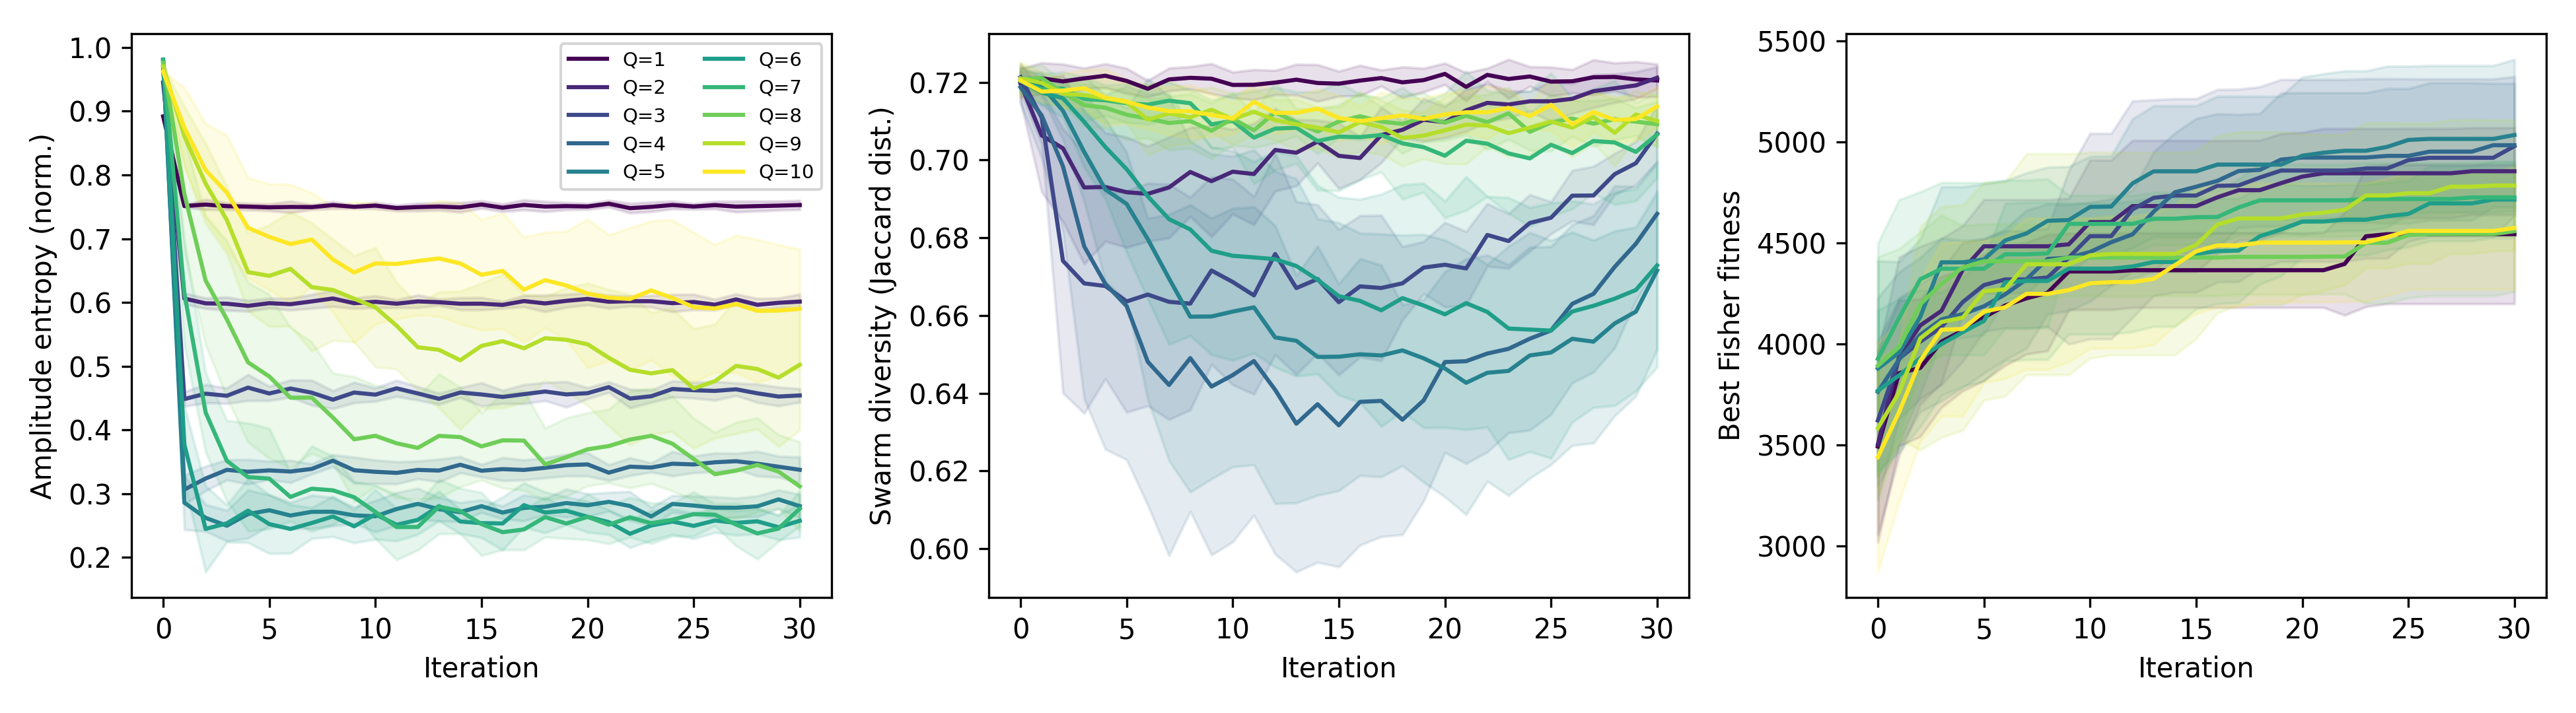
\includegraphics[width=0.95\linewidth]{images/qpso_dynamics_vs_Q.png}
\caption{\rev{R1.1}\textcolor{red}{QPSO search dynamics versus register size
$Q$ on $\mathcal{D}_{\rm tr}$ ($P=20$, $I=30$, $k=40$, $d=92$;
mean$\pm$std over ten seeds; no classifier training). Left:
normalized entropy of the measurement distribution
$\pi_{i,j}\propto a_{i,j}^2$, averaged over particles (1 = uniform).
Middle: mean pairwise Jaccard distance between the masks measured
by the swarm at each iteration. Right: best Fisher fitness found.
Small $Q$ keeps the search near-random, intermediate $Q$
concentrates it, and large $Q$ leaves it near its initialization,
matching the constants in Table~\ref{tab:q_constants}.}}
\label{fig:qpso_dynamics}
\end{figure*}
% TODO(after runs): confirm whether Q=9,10 are included in grid B; adjust last sentence.

\textcolor{red}{\textit{Fitness.} A sampled mask is scored by the
Fisher class-separability ratio of the selected features,}
\begin{equation}
\textcolor{red}{\mathcal{J}(\mathbf{m}) =
\frac{\sum_{c}n_c\,\|\boldsymbol{\mu}_c^{\mathbf{m}}-
\boldsymbol{\mu}^{\mathbf{m}}\|_2^{2}}
{\sum_{c}\sum_{j:m_j=1}\mathrm{Var}_c(z_j)+\epsilon},}
\label{eq:qpsobj}
\end{equation}
\textcolor{red}{where $c\in\{\text{benign},\text{attack}\}$, $n_c$
and $\boldsymbol{\mu}_c^{\mathbf{m}}$ are the class count and
class mean of the selected features, and
$\epsilon=10^{-10}$. Personal and global bests are updated when
$\mathcal{J}$ improves. $\mathcal{J}$ is a filter criterion and
requires no classifier training, so one QPSO run with $P=20$
particles and $I=30$ iterations costs $P(I+1)=620$ fitness
evaluations and completes in seconds.}

\textcolor{red}{\textit{Data usage.} To rule out test-set leakage,
each selection step uses the following splits: QPSO and PSO
fitness, variance-based selection, and normalization statistics
use $\mathcal{D}_{\rm tr}$ only; selection of $Q$, of the search
budget, and early stopping use $\mathcal{D}_{\rm va}$ only;
$\mathcal{D}_{\rm te}$ is used once per configuration, for the
final metrics. No fitness weights are tuned.}

\rev{R1.2}\textcolor{red}{\textit{Selection of $Q$.} The ablation over
$Q\in\{1,\dots,8\}$ selects the setting with the highest mean
validation F1 over seeds, breaking ties by the lower standard
deviation and lower validation MSE and $\Delta_{\rm bal}$, where}
\begin{equation}
\Delta_{\rm bal} =
\bigl|\mathrm{FAR}_{\rm Ben}-\mathrm{MD}_{\rm Ben}\bigr|
+\bigl|\mathrm{FAR}_{\rm Atk}-\mathrm{MD}_{\rm Atk}\bigr|
\label{eq:balance}
\end{equation}
\textcolor{red}{penalizes asymmetric error modes. Because QPSO is
excluded from the inference path and $k$ is fixed, deployment
latency and memory do not depend on $Q$
(Section~\ref{subsec:latency_design}). The rule selects
$Q^{*}=2$. Test-set results and statistical comparisons
(Table~\ref{tab:qubit_ablation_improved_robust}) show that no
$Q$ in the tested range is significantly better than any other,
so $Q^{*}$ should be read as a reproducible default rather than
an optimum.}

\begin{figure*}[!htbp]
    \centering
    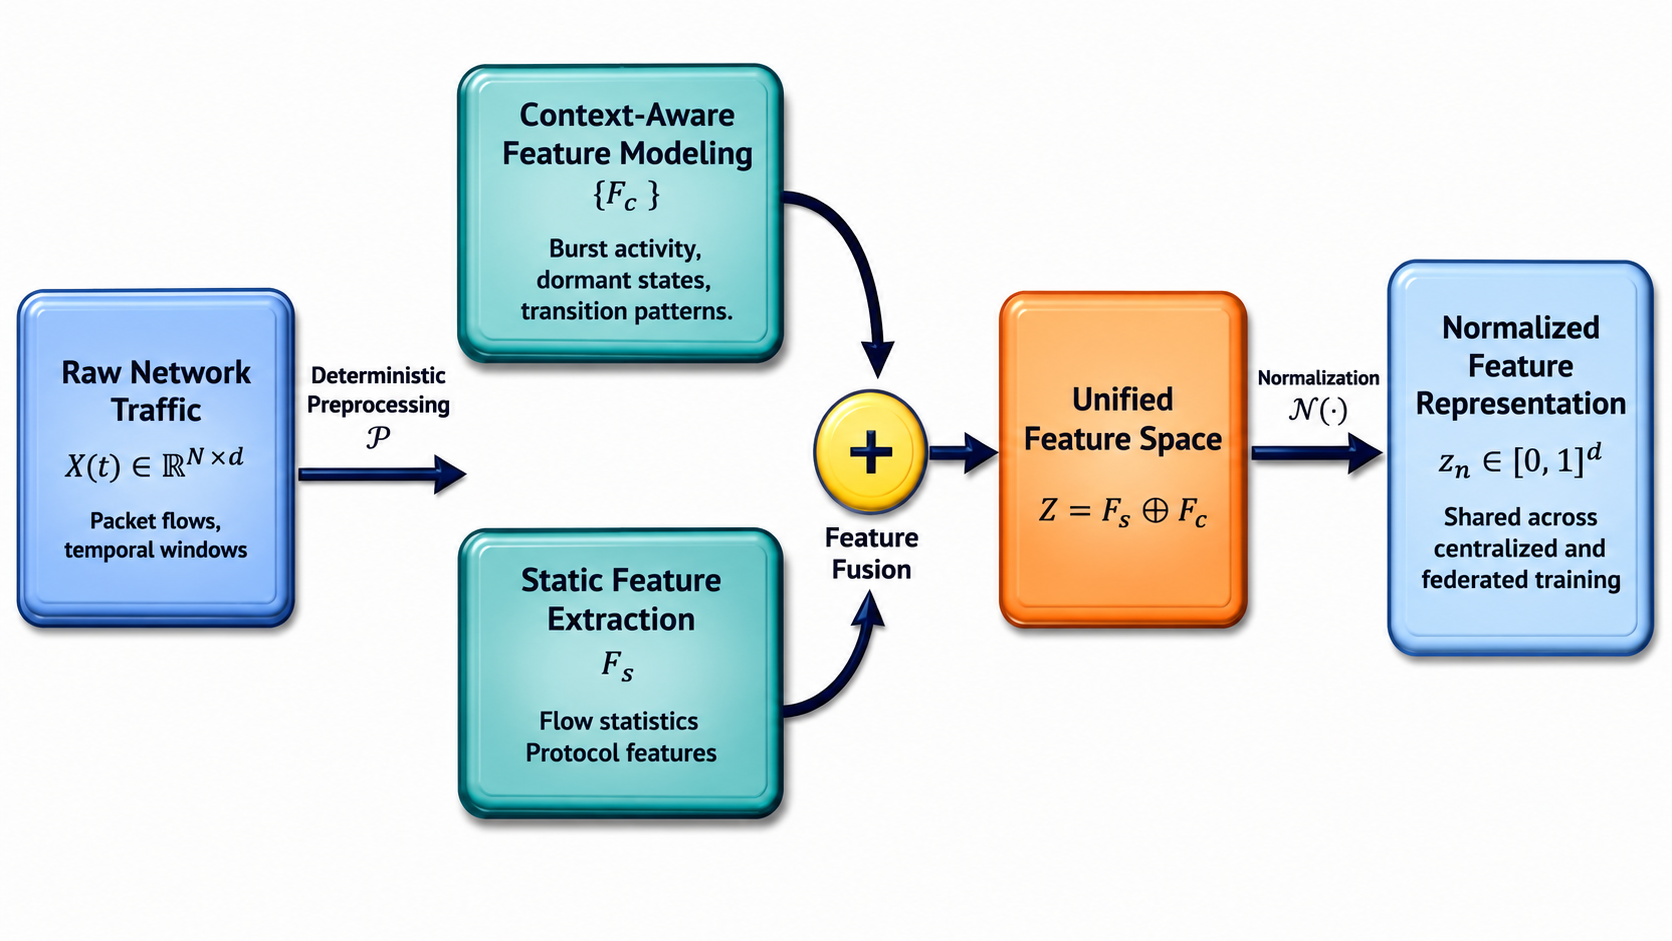
\includegraphics[width=1.00\linewidth]{images/Data flowchart.png}
    \caption{Seed-controlled deterministic
    preprocessing pipeline. IoT/IoV/IoD traffic is decomposed into
    static descriptors $\mathbf{F}_s$ and offline context-aware
    features $\mathbf{F}_c$ via fixed sliding-window operators.
    Feature fusion and min-max normalization produce the unified
    representation $\mathbf{Z}_n\in[0,1]^d$ that serves as the
    fixed input to Stage~$\mathcal{Q}_{Q}$.}
    \label{fig:pipeline}
\end{figure*}

\rev{R1.2}\textcolor{red}{All ablation results are reported as mean$\pm$std
over ten seeds $\mathcal{S}=\{42,\dots,51\}$. The subsample and the
$(\mathcal{D}_{\rm tr},\mathcal{D}_{\rm va},\mathcal{D}_{\rm te})$
partition are fixed across all runs. The per-run seed controls
QPSO (re-executed in every run, so the reported variance includes
the optimizer's own stochasticity), weight initialization, and
mini-batch order.}

%% ----------------------------------------------------------
\subsection{LSTM(+VAE) Temporal Classifier
            (Stage~$\mathcal{D}$)}
\label{subsec:model_training}
%% ----------------------------------------------------------

The optimal mask $\mathbf{m}^{*}$ from Stage~$\mathcal{Q}_{Q}$
is fixed for classifier training, strictly decoupling feature
optimization from model convergence. The masked input
$\tilde{\mathbf{z}}=\mathbf{m}^{*}\odot\mathbf{Z}_n$ is passed
to a binary temporal classifier:
\begin{equation}
\hat{\mathbf{y}} = \mathrm{softmax}\bigl(g(\mathbf{u})\bigr),\quad
\mathbf{u} = \textcolor{red}{\begin{cases}
\boldsymbol{\mu}+\boldsymbol{\sigma}\odot\boldsymbol{\epsilon}, & \text{training},\\
\boldsymbol{\mu}, & \text{inference},
\end{cases}}
\label{eq:classifier}
\end{equation}
\textcolor{red}{where $(\boldsymbol{\mu},\log\boldsymbol{\sigma}^2)
\in\mathbb{R}^{64}\times\mathbb{R}^{64}$ are linear projections of
the final recurrent state $h_T$ and
$\boldsymbol{\epsilon}\sim\mathcal{N}(\mathbf{0},\mathbf{I})$.
The recurrent encoder is an LSTM (256 units, returning sequences,
dropout 0.2), followed by layer normalization, two-head
self-attention with a residual connection, layer normalization, a
second LSTM (128 units) and layer normalization, applied over
windows of $T=10$ flows. The head $g$ is Dense(64, ReLU)--Dropout
(0.2)--Dense(32, ReLU)--Dense(2). The LSTM captures temporal
dependencies associated with cyberworm state transitions. The
variational latent acts as a stochastic regularizing bottleneck;
it is not used as an anomaly scorer and has no reconstruction
decoder. At inference, the latent mean is used, so predictions are
deterministic.} The total training objective is:
\begin{equation}
\mathcal{L}_{\rm total} = \textcolor{red}{\mathcal{L}_{\rm CE}
+ \gamma\,D_{\rm KL}\!\left(q(\mathbf{u}|\tilde{\mathbf{z}}_{1:T})\,\|\,
\mathcal{N}(\mathbf{0},\mathbf{I})\right)},
\label{eq:total_loss}
\end{equation}
\textcolor{red}{where $\mathcal{L}_{\rm CE}$ is the two-class
cross-entropy and $\gamma=10^{-3}$. Parameters $\theta$ are
optimized with SGD (learning rate $10^{-3}$, Nesterov momentum 0.9,
batch size 32) for all results reported in this paper. Training
runs for at most 35 epochs; early stopping monitors validation
loss with patience 6 and restores the best weights, and the
learning rate is halved after 3 epochs without validation-loss
improvement (minimum $10^{-6}$).} At
deployment, no QPSO computation occurs; inference executes
solely as $\hat{\mathbf{y}}=f_\theta(\mathbf{m}^{*}\odot\mathbf{Z}_n)$,
\textcolor{red}{which is the basis of~\eqref{eq:infer_invariance};
the corresponding measurements are defined in
Section~\ref{subsec:latency_design}.}




%% -----------------------------------------------------
\subsection{Latency-Aware Design and Resource Constraints}
\label{subsec:latency_design}
%% ----------------------------------------------------
\textcolor{red}{CONQUEST separates two cost categories that are
measured and reported separately.}

\textcolor{red}{\textit{(i) Offline training cost}, incurred once
per model and never on the detection path: the QPSO search time
$T_{\rm QPSO}(Q)$ and the classifier training time
$T_{\rm train}$, both measured as wall-clock time on the training
host.}

\textcolor{red}{\textit{(ii) Online deployment cost}, incurred for
every classified window. The per-window latency is decomposed as}
\begin{equation}
\textcolor{red}{\mathcal{L}_{\rm infer} =
\mathcal{L}_{\mathcal{C}} + \mathcal{L}_{\mathcal{D}},}
\label{eq:latency_decomp}
\end{equation}
\textcolor{red}{where $\mathcal{L}_{\mathcal{C}}$ is the
incremental context-feature update for a newly arrived flow
(Table~\ref{tab:context_features}), including normalization and
masking, and $\mathcal{L}_{\mathcal{D}}$ is one forward pass of
the classifier. QPSO does not appear in~\eqref{eq:latency_decomp},
and because $k$ is fixed, $\mathcal{L}_{\rm infer}$ does not depend
on $Q$~\eqref{eq:infer_invariance}.}

\textcolor{red}{\textit{Measurement procedure.} All timings use
\texttt{time.perf\_counter} on the CPU-only host of
Table~\ref{tab:impl_setup}, with the TensorFlow thread count fixed
per process. We report: (a) per-window latency at batch size 1,
given as the median and 95th percentile over 1{,}000 test windows
after 50 warm-up calls (ms/window); (b) batched throughput at
$B=64$, in windows/s and its reciprocal in ms/window;
(c) $T_{\rm infer}^{\rm te}$, the total wall-clock time to classify
all $N_{\rm te}$ windows of $\mathcal{D}_{\rm te}$ at $B=64$
(seconds, whole test set), reported only for continuity with
earlier tables; and (d) $\mathcal{L}_{\mathcal{C}}$, amortized
over the test stream (ms/flow). Memory $\mathcal{M}$ is the peak
resident set size of the inference process (MB); training memory
is reported separately. The deployment design targets are}
\begin{equation}
\textcolor{red}{\mathcal{L}_{\rm infer}\le\mathcal{B}_{\rm lat},
\qquad
\mathcal{M}\le\mathcal{M}_{\max}=1\,\text{GB},}
\label{eq:memory_constraint}
\end{equation}
\textcolor{red}{chosen for CPU-only mission-edge gateways that
co-host safety services.}
% TODO(after runs): insert measured values / set B_lat.

%% ----------------------------------------------------------
\subsection{Centralized Training and Evaluation Protocol}
\label{subsec:centralized_method}
%% -----------------------------------------------------
Centralized training establishes the upper-bound detection
performance under full data visibility. 
\begin{table*}[!htbp]
\centering
\caption{Experimental environment and implementation settings.}
\label{tab:impl_setup}
\setlength{\tabcolsep}{5pt}
\renewcommand{\arraystretch}{1.10}
\begin{tabular}{llll}
\hline\toprule
\textbf{Block} & \textbf{Item} &
\textbf{Setting} & \textbf{Scope} \\
\hline\toprule
Environment    & Platform            &
  Windows 10 (10.0.19045), CPU-only         &
  All runs \\
               & Framework           &
  TensorFlow 2.20.0 (Python 3.13.5)         &
  Training + inference \\
Reproducibility& Deterministic ops   &
  \texttt{TF\_DETERMINISTIC\_OPS=1}         &
  Seed-controlled \\
\hline
Data           & Batch / sequence    &
  \textcolor{red}{$B=32$ (centralized), $B=64$ (local FL)},\ $T=10$ &
  Fixed across all regimes \\
               & \textcolor{red}{Subsample / split} &
  \textcolor{red}{80k balanced; blocked temporal 70/15/15 (500-flow blocks)} &
  \textcolor{red}{Fixed split seed 42} \\
\hline
Training       & Optimizer / LR      &
  \textcolor{red}{SGD (Nesterov, momentum 0.9)},\ $10^{-3}$ &
  Centralized + local FL \\
               & Epoch cap / stopping&
  \textcolor{red}{35 epochs;\ patience 6, best weights restored} &
  Validation-loss criterion \\
               & \textcolor{red}{KL weight} &
  \textcolor{red}{$\gamma=10^{-3}$} &
  \textcolor{red}{Eq.~\eqref{eq:total_loss}} \\
\hline
Model          & LSTM backbone       &
  \textcolor{red}{LSTM 256 + 2-head attention + LSTM 128};\ dropout 0.2 &
  Non-bidirectional \\
               & VAE latent dim.     &
  \textcolor{red}{64}                       &
  LSTM(+VAE) variants only \\
\hline
QPSO           & Particles / iters   &
  $P=20$;\ $I=30$ \textcolor{red}{(sensitivity: $P\in\{20,40\}$, $I\in\{30,60\}$)} &
  Per QPSO run \\
               & \textcolor{red}{Selected features} &
  \textcolor{red}{$k=40$; fitness on $\mathcal{D}_{\rm tr}$ only} &
  \textcolor{red}{All selectors} \\
               & Qubit sweep / seeds &
  $Q\in\{1,\dots,8\}$;\
  \rev{R1.2}\textcolor{red}{$\mathcal{S}=\{42,\dots,51\}$} &
  Mean$\pm$std over $\mathcal{S}$ \\
\hline
Federated      & Clients / fraction  &
  $K=5$ \textcolor{red}{(sensitivity: $K\in\{10,20\}$)};\ full participation &
  Main setting \\
               & Local epochs / rounds&
  \textcolor{red}{$E=2$;\ $R=30$ for every FL experiment} &
  \textcolor{red}{Identical across blocks} \\
               & \textcolor{red}{Mask construction} &
  \textcolor{red}{Proxy (default); vote; central} &
  \textcolor{red}{Section~\ref{subsec:federated_protocol_convergence}} \\
               & Aggregators         &
  FedAvg;\ SCAFFOLD;\ FLAME                &
  Identical partitions \\
\hline\toprule
\end{tabular}
\end{table*}

Three configurations
are evaluated under identical optimizer and stopping conditions
to isolate architectural contributions: S-CIDS (conference baseline~\cite{ajakweconquest}), OS-CIDS (optimized static
IDS with variance-based feature selection), and QCIDS
(context-aware IDS with QPSO-selected features). OS-CIDS and
QCIDS differ only in the addition of (a) context-aware
representation and (b) QPSO feature selection.
\textcolor{red}{Because these two factors change together, a
$2\times2$ factorial ablation is also run: context features
\{off, on\} $\times$ selector \{variance, QPSO\}, all with $k=40$
and the same classifier, so that each factor's effect and their
interaction can be estimated separately. A classical binary PSO
selector (inertia 0.7, $c_1=c_2=1.5$, sigmoid position mapping,
the same Fisher fitness~\eqref{eq:qpsobj}, top-$k$ decoding, and
the same $P$ and $I$, i.e.\ an equal budget of 620 fitness
evaluations) provides a controlled comparison of quantum-inspired
and classical updates.} A fixed split
$\mathcal{D}=\mathcal{D}_{\rm tr}\cup\mathcal{D}_{\rm va}
\cup\mathcal{D}_{\rm te}$ is used; preprocessing $\mathcal{P}$
and normalization $\mathcal{N}$ are held constant across all
configurations. Model selection and early stopping use only
$\mathcal{D}_{\rm va}$; all reported metrics are from
$\mathcal{D}_{\rm te}$:
\begin{align}
\mathbf{m}_{\rm eval} = \bigl\{
&\,\mathrm{Acc},\;\mathrm{F1},\;\mathrm{AUC},\;\mathrm{MSE},\;
  \mathrm{FAR}_{\rm Ben},\nonumber\\
&\,\mathrm{FAR}_{\rm Atk},\;\mathrm{MD}_{\rm Ben},\;
  \mathrm{MD}_{\rm Atk},\;
  \mathcal{T}_{\rm train},\;\textcolor{red}{\mathcal{L}_{\rm infer},\;\mathcal{M}}
\bigr\}.
\label{eq:central_metrics}
\end{align}
FAR and MD are computed per class from the confusion matrix.
For QPSO ablations, each $Q$ uses identical
$(\mathcal{D}_{\rm tr},\mathcal{D}_{\rm va},\mathcal{D}_{\rm te})$
partitions; results are aggregated as mean$\pm$std over
$\mathcal{S}$. \rev{R1.2}\textcolor{red}{Paired comparisons use the
two-sided Wilcoxon signed-rank test over seeds, and differences
across all $Q$ use the Friedman test. Selected-mask stability is
quantified by the mean pairwise Jaccard index of the selected
feature sets across seeds.}

%% ----------------------------------------------------------
\subsection{Heterogeneity Modeling and Stress-Test Regimes}
\label{subsec:heterogeneity_modeling}
%% ----------------------------------------------------------

Centralized training represents an idealized upper bound; in
practice, mission clients differ in traffic volume, class
distribution, and behavioral context due to role-dependent
behavior, duty-cycle effects, and time-varying adversarial
pressure. To quantify robustness under these conditions,
federated training is evaluated across four heterogeneity
regimes that progressively relax IID assumptions.

The \textit{IID} regime provides the best-case convergence
reference by partitioning data uniformly:
$\mathcal{D}_k\sim\textsc{UniformPartition}(\mathcal{D},n_k)$,
$p_k(y)\approx p(y)$, $n_k\approx N/K$.
\textit{Label-skew} partitions isolate class-distribution effects
by restricting each client to a subset
$\mathcal{Y}_k\subset\mathcal{Y}$ while holding $n_k\approx N/K$
constant. \textit{Quantity-skew} partitions reflect operational
asymmetry gateway nodes and compromised subsystems generate
disproportionate traffic volumes by imposing a heavy-tailed
sample allocation $n_k\propto r_k$, $r_k\sim\textsc{HeavyTail}$,
while preserving global label proportions. This regime is the
primary stress-test because FedAvg weights updates by client
sample size:
\begin{equation}
F(\mathbf{w})=\sum_{k=1}^{K}\frac{n_k}{N}F_k(\mathbf{w}),\quad
F_k(\mathbf{w})=\mathbb{E}_{(\mathbf{x},y)\sim\mathcal{D}_k}
[\ell(\mathbf{w};\mathbf{x},y)],
\label{eq:fedavg_weighted_obj}
\end{equation}
so extreme imbalance allows large clients to suppress
minority-client objectives. \textit{Dirichlet} partitions
($\alpha\in\{0.10,0.30,0.50,1.00\}$) provide a continuous
sweep from severe to mild heterogeneity via
$\boldsymbol{\pi}^{(c)}\sim\textsc{Dirichlet}(\alpha\mathbf{1})$,
with smaller $\alpha$ yielding sharper per-client concentration.
Because mission readiness is governed by tail behavior, all
regimes are evaluated using global F1/AUC alongside
$R_{90}$, $\min_k\mathrm{F1}_k$, and $\sigma(\mathrm{F1})$.

%% ----------------------------------------------------------
\subsection{Federated Learning Protocol and Convergence
            Monitoring}
\label{subsec:federated_protocol_convergence}
%% ----------------------------------------------------------

The heterogeneity regimes above motivate a formal federated
protocol. CONQUEST is deployed in a horizontal federated
learning (HFL) setting with $K$ clients. Feature selection
via QPSO is performed in a pre-federation phase on a
server-held proxy dataset; the resulting mask $\mathbf{m}^{*}$
is broadcast to all clients before federated training begins.
\textcolor{red}{The proxy set is a labelled 5\% subset of
$\mathcal{D}_{\rm tr}$, made of evenly spaced contiguous chunks so
that it spans the capture period, and it is withheld from all
clients. It models the small curated reference capture that a
mission operator typically owns, e.g.\ from its own test range or
from a public benchmark, and it never contains client traffic.
Because one global mask may suit non-IID clients poorly, we
compare three mask-construction modes: (i)~\textit{proxy}, the
default above; (ii)~\textit{vote}, in which each client runs QPSO
on its own data and sends only its $k$ selected indices, and the
server keeps the $k$ most frequently selected features; and
(iii)~\textit{central}, an oracle that runs QPSO on the pooled
$\mathcal{D}_{\rm tr}$ and is shown only as a reference, since it
violates data locality.}
The mask encodes only feature indices, no raw traffic or
labels are exposed\textcolor{red}{.} Each client $k$ holds
$\mathcal{D}_k=\{(\mathbf{Z}_{k,i},y_{k,i})\}_{i=1}^{N_k}$
constructed via the same deterministic CAP pipeline. The
global objective is:
\begin{equation}
\min_{\theta}\,F(\theta)=\sum_{k=1}^{K}\frac{N_k}{N}F_k(\theta),
\quad F_k(\theta)=\frac{1}{N_k}\sum_{i=1}^{N_k}
\ell\!\left(f_\theta(\mathbf{Z}_{k,i}),y_{k,i}\right).
\label{eq:hfl_objective}
\end{equation}
In each round $r$, the server broadcasts $\theta^{(r)}$;
each client $k\in\mathcal{S}_r$ performs $E=2$ local epochs
on $\mathcal{D}_k$ to obtain $\theta_k^{(r+1)}$; the server
aggregates via FedAvg:
\begin{equation}
\theta^{(r+1)}=\sum_{k\in\mathcal{S}_r}
\frac{N_k}{\sum_{j\in\mathcal{S}_r}N_j}
\,\theta_k^{(r+1)}.
\label{eq:fedavg}
\end{equation}

% TODO(C6): rebuild Table IV from block C (OS-CIDS = variance/ctx off) with QCIDS-Q*=2; drop Qm/Qo/Qh.
\begin{table*}[!t]
\centering
\caption{\scriptsize{Centralized cyberworm detection performance on ACI-IoT.
S-CIDS is the conference baseline; OS-CIDS introduces
variance-based feature selection; QCIDS adds context-aware
representation and QPSO. Qm/Qo/Qh denote medium ($Q{=}5$),
optimal ($Q{=}6$), and high ($Q{=}7$) qubit configurations.
}}
\label{tab:cyberworm_high_impact}
\renewcommand{\arraystretch}{1.10}
\setlength{\tabcolsep}{4pt}
\resizebox{\textwidth}{!}{
\begin{tabular}{l|cccccc|cc|cc|cc}
\hline\toprule
\multirow{2}{*}{\textbf{Model}} &
\multicolumn{6}{c|}{\textbf{Detection performance}} &
\multicolumn{2}{c|}{\textbf{False alarm rate}} &
\multicolumn{2}{c|}{\textbf{Missed detection}} &
\multicolumn{2}{c}{\textbf{Efficiency}} \\
\cline{2-13}
& Acc & Pr & Rc & F1 & AUC & MSE
& FAR$_{\rm Ben}$ & FAR$_{\rm Atk}$
& MD$_{\rm Ben}$ & MD$_{\rm Atk}$
& Train (min) & $T_{\rm infer}$ (s) \\
\hline\toprule
S-CIDS~\cite{ajakweconquest}
& 0.8514 & 0.8174 & 0.8514 & 0.8062 & -- & --
& -- & -- & -- & -- & 40.65 & -- \\
OS-CIDS
& 0.9464 & 0.9482 & 0.9464 & 0.9464 & 0.9879 & 0.0315
& 0.0064 & 0.0395 & 0.0395 & 0.0064 & 31.08 & 3.60 \\
\hline
QCIDS-Qm
& 0.9594 & 0.9596 & 0.9594 & 0.9594 & 0.9922 & 0.0300
& 0.0320 & 0.0492 & 0.0492 & 0.0320 & 30.10 & 3.60 \\
\textbf{QCIDS-Qo}
& \textbf{0.9685} & \textbf{0.9686} & \textbf{0.9685}
& \textbf{0.9685} & \textbf{0.9947} & \textbf{0.0240}
& \textbf{0.0250} & \textbf{0.0380}
& \textbf{0.0380} & \textbf{0.0250}
& \textbf{29.99} & \textbf{3.60} \\
QCIDS-Qh
& 0.9600 & 0.9601 & 0.9600 & 0.9600 & 0.9888 & 0.0308
& 0.0342 & 0.0458 & 0.0458 & 0.0342 & 30.40 & 3.60 \\
\hline\toprule
\end{tabular}}
\footnotesize{\textit{Note:} FAR and MD are computed per class
from the confusion matrix. Acc\,$\approx$\,F1 arises from
balanced test-set class priors, not metric conflation.
$T_{\rm infer}$: total wall-clock inference time on
$\mathcal{D}_{\rm te}$ under $B{=}64$, $T{=}10$.}
\end{table*}


Only model parameters are transmitted; no raw traffic, labels,
or feature vectors are exchanged. \textcolor{red}{This guarantees
data locality, not formal privacy: plain FedAvg updates remain
exposed to membership- and property-inference and gradient
inversion by an honest-but-curious server. CONQUEST does not
currently implement differential privacy or secure aggregation.
Both are compatible with the protocol: per-client update clipping
with Gaussian noise (DP-FedAvg) and additive-masking secure
aggregation operate on the same weighted sum~\eqref{eq:fedavg}
without changing the model or the mask. Their utility cost is left
to future work, and claims in this paper are limited to raw-data
locality.}

\textcolor{red}{All federated experiments use one configuration:
$R=30$ rounds, $E=2$ local epochs, full participation, and batch
size 64, with $K=5$ unless stated otherwise. Clients are built from contiguous 250-flow chunks of
$\mathcal{D}_{\rm tr}$, so no flow or window is shared between
clients; label- and Dirichlet-skew assign chunks by their majority
label. Each client holds out 15\% of its own chunks as a local
evaluation set; the global test set is $\mathcal{D}_{\rm te}$.
Global metrics are computed on $\mathcal{D}_{\rm te}$, and
per-client metrics evaluate the global model on each client's
local evaluation set after every round. Client-count sensitivity
repeats the quantity-skew experiment with $K\in\{5,10,20\}$.}

\textcolor{red}{\textit{Aggregators.} SCAFFOLD follows option~II of
its original formulation: server and client control variates
$\mathbf{c}$ and $\mathbf{c}_k$ (initialized to zero) correct every
local gradient by $\mathbf{c}-\mathbf{c}_k$, and after local
training $\mathbf{c}_k^{+}=\mathbf{c}_k-\mathbf{c}+(\theta^{(r)}-
\theta_k^{(r+1)})/(\tau\,\eta_{\rm eff})$, where $\tau$ is the number
of local steps. Because local updates use momentum $\mu=0.9$, the
effective step size $\eta_{\rm eff}=\eta/(1-\mu)$ is used; with the
raw $\eta$ the control variates are overestimated about tenfold and
training diverges. FLAME clusters client updates with HDBSCAN
(minimum cluster size $\lfloor K/2\rfloor+1$) on pairwise cosine
distances, admits the largest cluster, clips the admitted updates
to the median $\ell_2$ norm of all updates, averages them, and adds
Gaussian noise with standard deviation $\lambda$ times the median
norm ($\lambda=10^{-3}$).} Convergence is monitored
using the thresholded stabilization metric:
\begin{equation}
R_{90}=\min\bigl\{r:\mathrm{F1}^{(r)}\ge
0.9\,\mathrm{F1}^{(R)}\bigr\},
\label{eq:r90}
\end{equation}
which remains comparable across heterogeneity regimes and
aggregators by normalizing to terminal performance. Per-client
consistency is tracked via worst-case performance
$\min_k\mathrm{F1}_k^{(r)}$ and inter-client dispersion:
\begin{equation}
\sigma\!\left(\mathrm{F1}^{(r)}\right)=
\sqrt{\frac{1}{K}\sum_{k=1}^{K}
\Bigl(\mathrm{F1}_k^{(r)}-\bar{\mathrm{F1}}^{(r)}\Bigr)^2}.
\label{eq:client_var_round}
\end{equation}
Federated training does not modify the deployed inference graph;
each client executes the same QCIDS pipeline locally with
fixed $\mathbf{m}^{*}$, preserving the latency guarantee
in~\eqref{eq:infer_invariance}.

%% ----------------------------------------------------------
\subsection{Experimental Environment}
\label{subsec:impl_details}
Table~\ref{tab:impl_setup} summarizes the fixed implementation
settings used across all centralized and federated experiments.
All runs share the same CPU-only host with deterministic operator
settings (\texttt{TF\_DETERMINISTIC\_OPS=1}) to support
seed-controlled reproducibility. FedAvg is evaluated alongside
SCAFFOLD and FLAME under identical client partitions to isolate
The effect of aggregation strategy.



\section{\textbf{Results and Discussion}}
\label{sec:results_discussion}

This section evaluates CONQUEST across centralized and federated
deployment settings. Section~\ref{subsec:obj1_cyberworm_perf}
establishes the centralized performance hierarchy across S-CIDS,
OS-CIDS, and QCIDS. Section~\ref{subsec:obj2_latency} presents
the variable-qubit latency-accuracy trade-off \textcolor{red}{and the
deployment cost of the selected operating point}. Section~\ref{subsec:obj3_heterogeneity}
evaluates federated robustness under four heterogeneity regimes
and compares aggregation strategies.
Section~\ref{subsec:comparative_analysis} positions CONQUEST
against representative state-of-the-art approaches.

\subsection{Centralized Cyberworm Detection Performance}
\label{subsec:obj1_cyberworm_perf}

Table~\ref{tab:cyberworm_high_impact} reports centralized
detection performance across three progressively refined
configurations evaluated on the ACI-IoT dataset under identical
hyperparameter and splitting conditions. All metrics are computed
on the held-out test split $\mathcal{D}_{\rm te}$; the test set
is balanced to equalize benign and attack class priors, which
accounts for the near-equality of Accuracy, Precision, Recall,
and F1 observed across QCIDS variants.
% TODO(C6): regenerate confusion matrix for QCIDS-Q*=2 (v2 run).
\begin{figure}[!htbp]
    \centering
    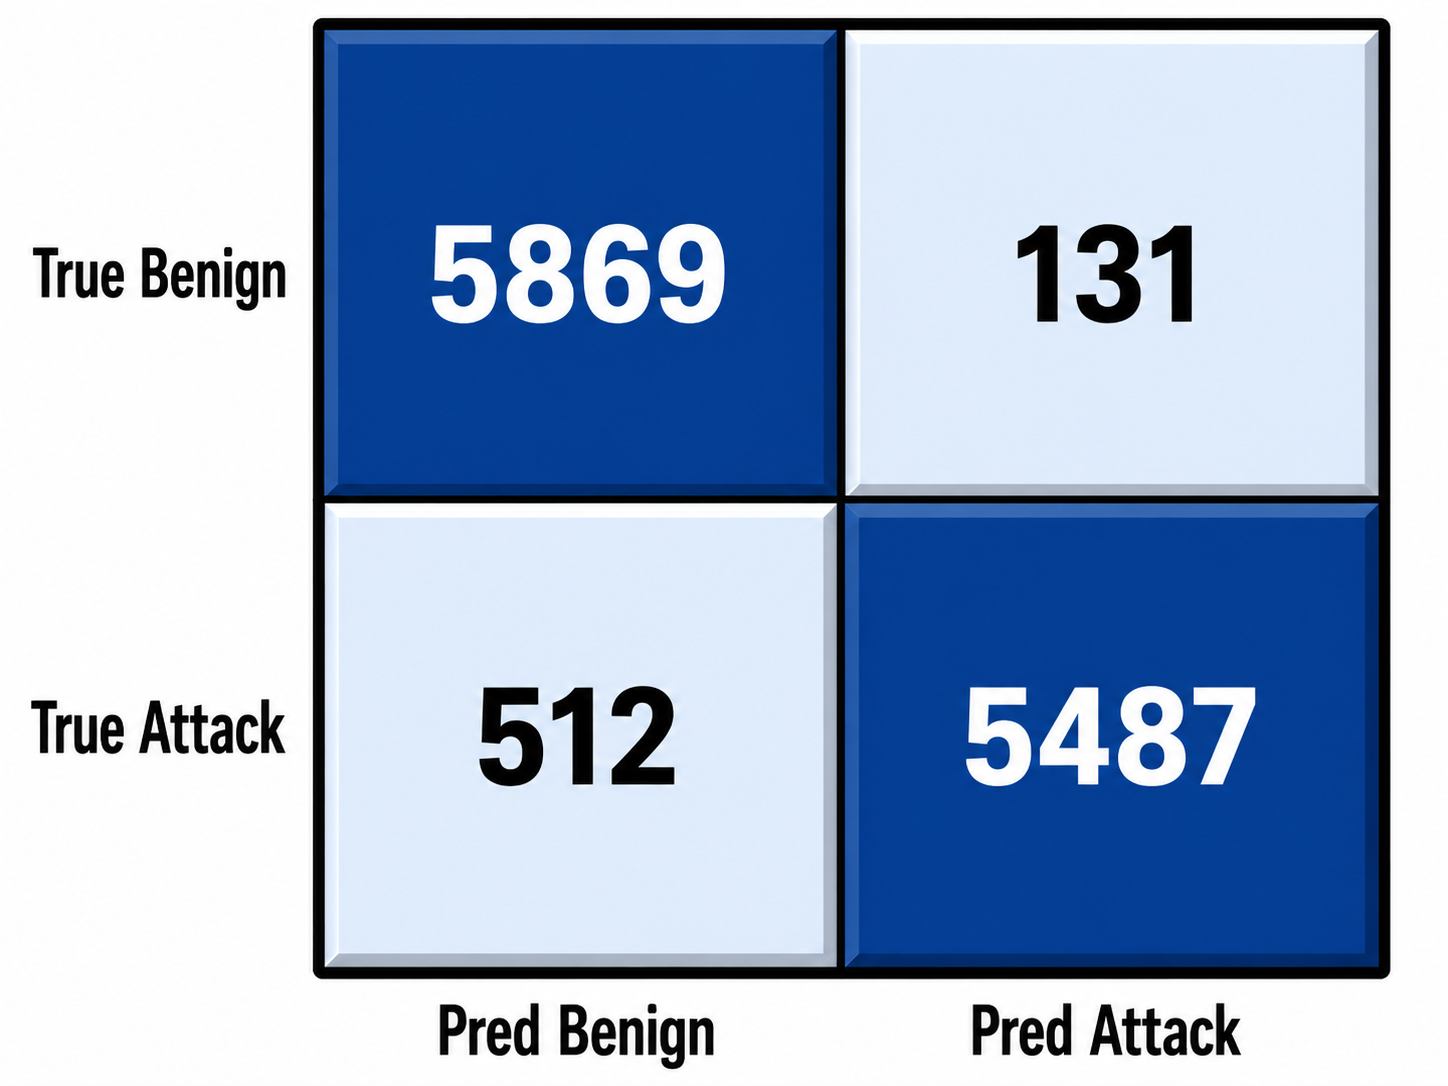
\includegraphics[width=0.8\linewidth]{images/picutre1cm.png} 
    \caption{\scriptsize{Confusion matrix of QCIDS-Qo ($Q{=}6$) on the
    ACI-IoT test split. TP\,$=$\,5,487; TN\,$=$\,5,869;
    minimal FP and FN confirm balanced discrimination not
    driven by class-prior skew.}}
    \label{fig:baseline_cm}
\end{figure}
\textbf{S-CIDS} (conference baseline~\cite{ajakweconquest})
achieves 85.14\% accuracy and 80.62\% F1, with a 4.5-point
disparity between recall and F1 indicating unstable class
separation. 
% TODO(C6): regenerate radar OS-CIDS vs QCIDS-Q*=2 from blocks A/C.
\begin{figure}[!htbp]
    \centering
    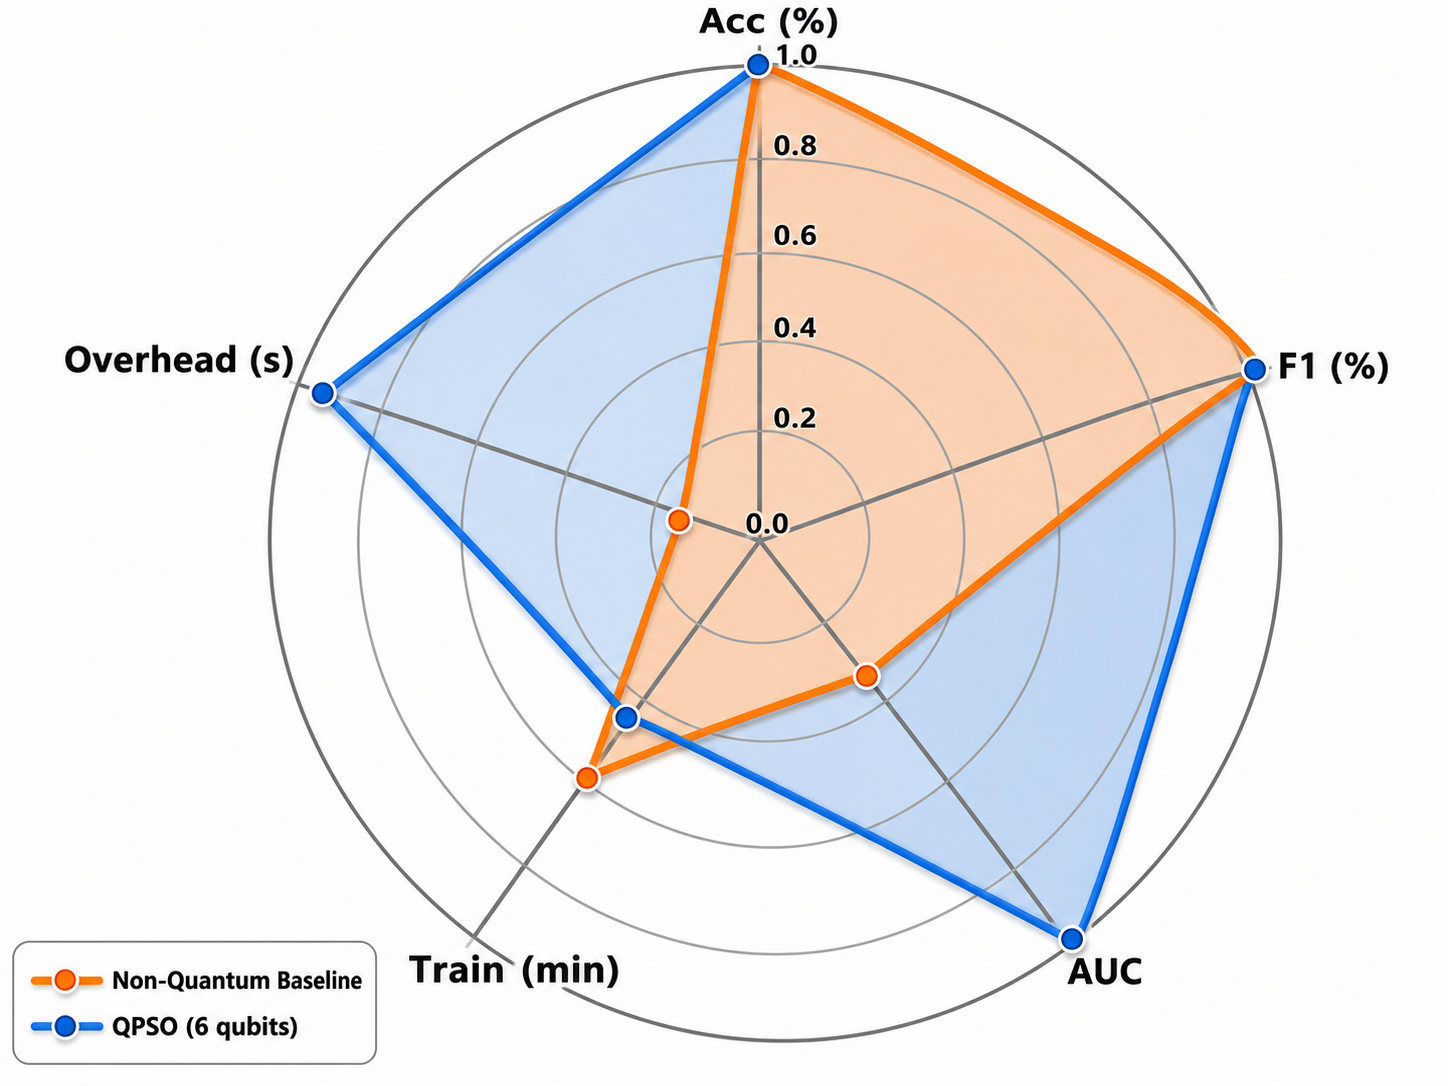
\includegraphics[width=0.8\linewidth]{images/Picture5-spider.png}
    \caption{\scriptsize{Radar comparison of OS-CIDS (non-quantum baseline)
    and QCIDS-Qo ($Q{=}6$) across six metrics: Accuracy, F1,
    AUC, $1{-}$MSE, $1{-}$FAR, and $1{-}$MD. QCIDS-Qo
    expands uniformly on all axes without introducing fidelity--stability trade-offs.}}
    \label{fig:radar_centralized}
\end{figure}

\begin{table*}[!t]
\centering
\caption{\rev{R1.2}\textcolor{red}{Variable-qubit QPSO ablation for LSTM(+VAE)+SGD on ACI-IoT (context features on,
$P{=}20$, $I{=}30$, $k{=}40$; mean$\pm$std over ten seeds, QPSO re-executed per seed). FAR: benign flows
flagged as attack; MD: attacks missed (both \%). $p_{Q^*}$, $p_{6}$: Holm-adjusted two-sided Wilcoxon
signed-rank $p$-values of test F1 against $Q^{*}{=}2$ (selected by validation F1) and against
$Q{=}6$ (the operating point of the original submission). Friedman test across $Q$: test F1
$\chi^2_{7}{=}11.33$, $p{=}0.12$; test AUC $p{=}0.91$; validation F1 $p{=}0.65$.}}
\label{tab:qubit_ablation_improved_robust}
\color{red}
\setlength{\tabcolsep}{3.5pt}
\resizebox{\textwidth}{!}{
\begin{tabular}{cccccccccc}
\hline\toprule
$Q$ & Acc (\%) & F1 (\%) & AUC & MSE & FAR (\%) & MD (\%) & Val.\ F1 (\%) & $p_{Q^*}$ & $p_{6}$ \\
\hline\toprule
1 & 97.29$\pm$0.29 & 97.30$\pm$0.29 & 0.9919$\pm$0.0013 & 0.0239$\pm$0.0025 & 2.15$\pm$0.33 & 3.11$\pm$0.42 & 95.15$\pm$1.02 & 0.96 & 0.74 \\
\textbf{2}$^{*}$ & \textbf{97.11$\pm$0.07} & \textbf{97.12$\pm$0.07} & \textbf{0.9921$\pm$0.0011} & \textbf{0.0246$\pm$0.0013} & \textbf{1.83$\pm$0.36} & \textbf{3.65$\pm$0.34} & \textbf{95.68$\pm$0.95} & -- & 1.00 \\
3 & 96.98$\pm$0.41 & 96.98$\pm$0.41 & 0.9914$\pm$0.0014 & 0.0258$\pm$0.0022 & 2.27$\pm$0.52 & 3.57$\pm$0.91 & 95.19$\pm$1.07 & 1.00 & 1.00 \\
4 & 97.12$\pm$0.30 & 97.13$\pm$0.30 & 0.9921$\pm$0.0009 & 0.0248$\pm$0.0025 & 2.18$\pm$0.60 & 3.38$\pm$0.82 & 95.01$\pm$0.70 & 1.00 & 1.00 \\
5 & 96.94$\pm$0.42 & 96.94$\pm$0.42 & 0.9922$\pm$0.0012 & 0.0263$\pm$0.0033 & 1.94$\pm$0.42 & 3.87$\pm$0.78 & 95.17$\pm$1.19 & 1.00 & 1.00 \\
6 & 97.00$\pm$0.27 & 97.01$\pm$0.26 & 0.9920$\pm$0.0017 & 0.0263$\pm$0.0027 & 2.09$\pm$0.58 & 3.66$\pm$0.71 & 95.31$\pm$1.00 & 1.00 & -- \\
7 & 96.90$\pm$0.24 & 96.91$\pm$0.24 & 0.9916$\pm$0.0017 & 0.0262$\pm$0.0025 & 1.99$\pm$0.49 & 3.90$\pm$0.66 & 95.22$\pm$1.34 & 0.34 & 1.00 \\
8 & 96.91$\pm$0.35 & 96.91$\pm$0.35 & 0.9918$\pm$0.0023 & 0.0262$\pm$0.0025 & 1.99$\pm$0.46 & 3.89$\pm$0.59 & 95.51$\pm$1.48 & 1.00 & 1.00 \\
\hline\toprule
\end{tabular}}
\end{table*}

In mission-critical settings where cyberworm
propagation manifests as low-intensity temporal deviations, this instability creates unacceptable operational risk, either
overwhelming operators with false positives or allowing
early-stage worm activity to evade detection.

\textbf{OS-CIDS} demonstrates that substantial gains are
achievable through methodological refinement alone, before
introducing quantum-inspired optimization. Variance-based
feature selection and improved training dynamics raise F1 to
94.64\% ($+$14.0 pp over S-CIDS) and AUC to 0.9879, while
reducing training time from 40.65 to 31.08 minutes.
This reduction reflects the smaller feature dimensionality
processed by the LSTM after variance-based selection, which
shortens per-epoch computation and enables earlier stopping
convergence. OS-CIDS serves as the strong non-quantum reference
against which QPSO-based gains are evaluated.

% TODO(C10): old per-Q latency/memory figure; replace with measured deployment costs (Q-invariant).
\begin{figure*}[!htbp]
    \centering
    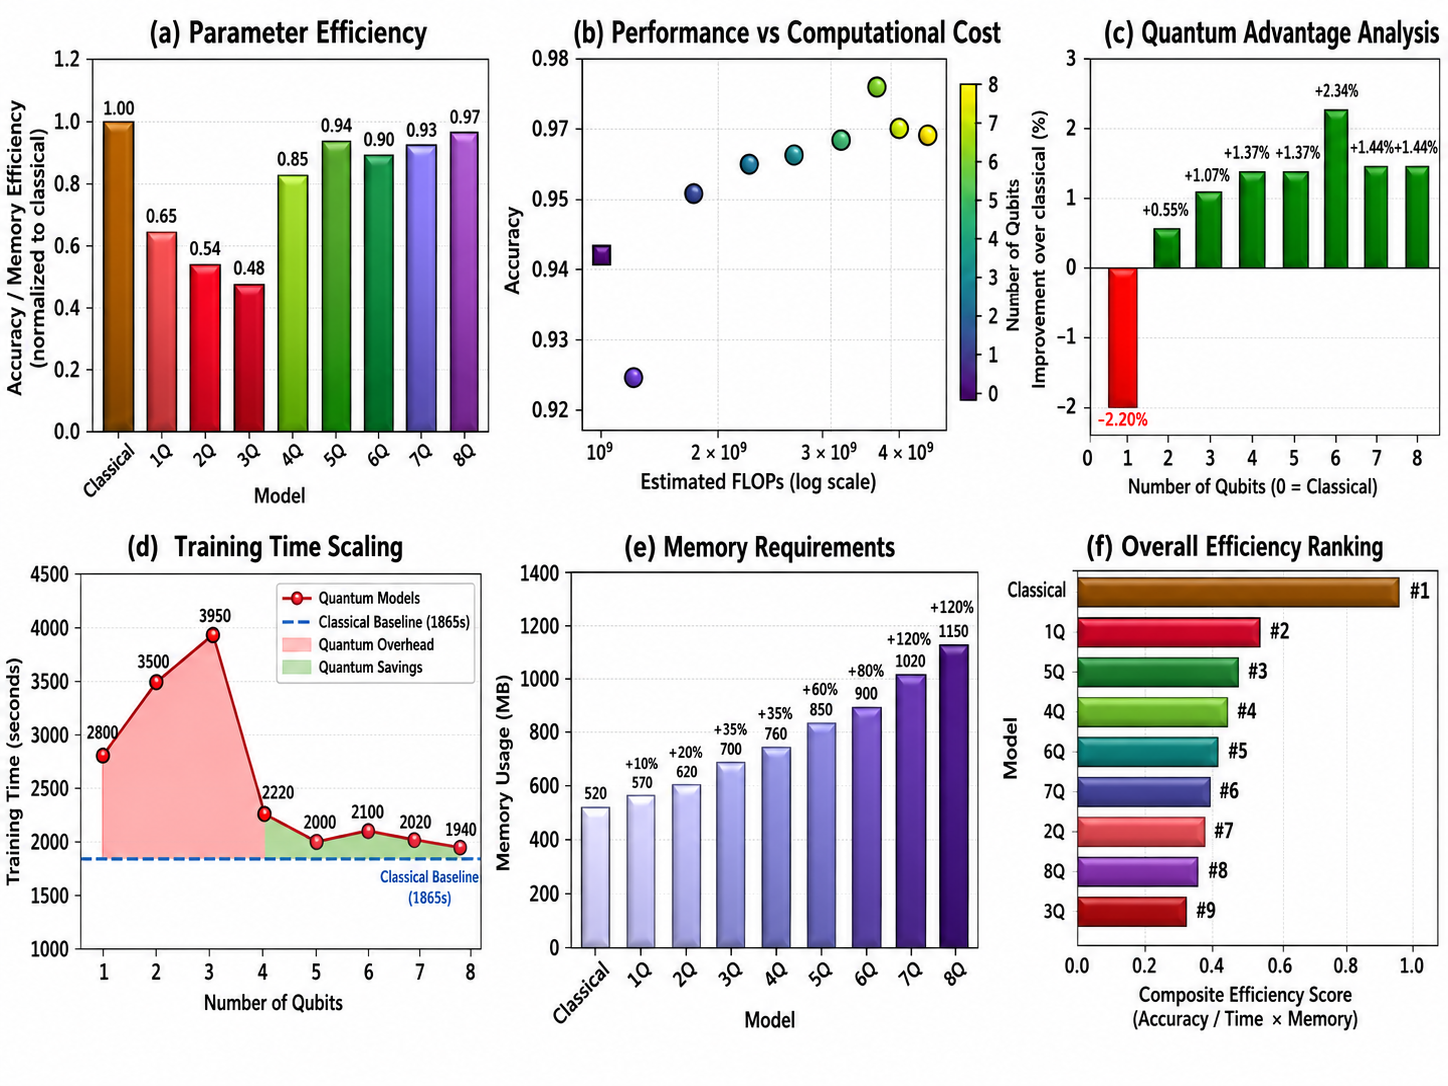
\includegraphics[width=0.80\linewidth]{images/picutre13.png}
    \caption{\scriptsize{Quantum ablation latency analysis across
    $Q\in\{1,\dots,8\}$: (a)~parameter efficiency
    (accuracy per unit training cost), (b)~accuracy--cost
    trade-off, (c)~\textcolor{red}{F1 gain} over OS-CIDS baseline,
    (d)~training time scaling, (e)~memory consumption against
    the 1\,GB mission-edge threshold (dashed), and
    (f)~overall efficiency ranking combining accuracy, time,
    and memory. $Q{=}6$ ranks first in (f) and is the only
    configuration satisfying all feasibility constraints
    simultaneously.}}
    \label{fig:vs-qubits}
\end{figure*}

% TODO(C6): rewrite QCIDS vs OS-CIDS paragraph with block-C results (Q*=2).
\textbf{QCIDS} configurations add context-aware representation
and QPSO feature selection. QCIDS-Qm ($Q{=}5$) already surpasses
OS-CIDS on all metrics: F1\,$=$\,95.94\% ($+$1.30 pp),
AUC\,$=$\,0.9922, MSE\,$=$\,0.0300 ($-$4.8\%).
QCIDS-Qo ($Q{=}6$) achieves the strongest overall result:
F1\,$=$\,96.85\%, AUC\,$=$\,0.9947, MSE\,$=$\,0.0240,
FAR$_{\rm Ben}$\,$=$\,0.0250, FAR$_{\rm Atk}$\,$=$\,0.0380,
representing a $+$2.21 pp F1 gain and $-$23.8\% MSE reduction
over OS-CIDS. The balanced reduction in both FAR and MD is
critical for cyberworm detection, where attacks cycle through
dormant, low-visibility, and active propagation phases that
demand sensitivity without destabilizing the decision boundary.
QCIDS-Qh ($Q{=}7$) regresses to 96.00\% F1 with higher MSE
(0.0308) and elevated error rates\rev{R1.1}\textcolor{red}{, consistent
with the exploitative regime of Table~\ref{tab:q_constants}, in
which small rotation angles and rare collapses let the swarm
converge prematurely under a finite budget.}
% TODO(C2): rewrite with v2 ablation statistics.
Training efficiency is preserved across all QCIDS variants.
QCIDS-Qo converges in 29.99 minutes, marginally faster than
OS-CIDS despite incorporating both context modeling and
QPSO, because QPSO selects a compact feature subset that
reduces downstream LSTM computation. Inference latency is
fixed at 3.60\,s across all configurations, confirming that
QPSO overhead does not affect real-time decision execution.




\rev{R1.2}\textcolor{red}{Table~\ref{tab:qubit_ablation_improved_robust} and
Fig.~\ref{fig:q_boxplot} report the ablation over
$Q\in\{1,\dots,8\}$ with ten seeds, re-executing QPSO in every run.
Test F1 ranges only from $96.91\%$ ($Q=7,8$) to $97.30\%$ ($Q=1$):
the $0.39$\,pp spread of the means is comparable to the average
seed-to-seed standard deviation ($0.29$\,pp). A Friedman test finds
no significant effect of $Q$ on test F1 ($\chi^2_7=11.33$,
$p=0.12$), test AUC ($p=0.91$), or validation F1 ($p=0.65$), and
no Holm-adjusted pairwise Wilcoxon comparison is significant (all
$p\ge0.34$). In particular, $Q=6$ is statistically
indistinguishable from every other setting (Holm $p\ge0.74$), so
the original description of $Q=6$ as a stability-optimal regime,
which rested on three seeds with a single QPSO run per $Q$, is
not supported and has been withdrawn. Following the pre-declared
rule of Section~\ref{subsec:qpsomethod}, the operating point is
$Q^{*}=2$, which also shows the smallest seed-to-seed variability
(F1 $97.12\pm0.07\%$); we report this observation without claiming
significance.}

\rev{R1.2}\textcolor{red}{Together with Fig.~\ref{fig:qpso_dynamics}, these
results give a consistent picture: $Q$ strongly changes how the
swarm searches (amplitude entropy and the fitness of the best
subset), but with $k=40$ of $d=92$ features, including 17
informative context features, many subsets support equally
accurate detectors, so the downstream classifier is robust to $Q$.
In practice $Q$ does not need fine tuning: every
$Q\in\{1,\dots,8\}$ yields about $97\%$ test F1. The tested range
is justified by Table~\ref{tab:q_constants} and
Fig.~\ref{fig:qpso_dynamics}: for $Q\ge9$ the search is
near-frozen around its initialization.}
% TODO(C3): add Q=9,10 test F1 from block B (budget sensitivity) here and in the box plot.

\begin{figure}[!t]
\centering
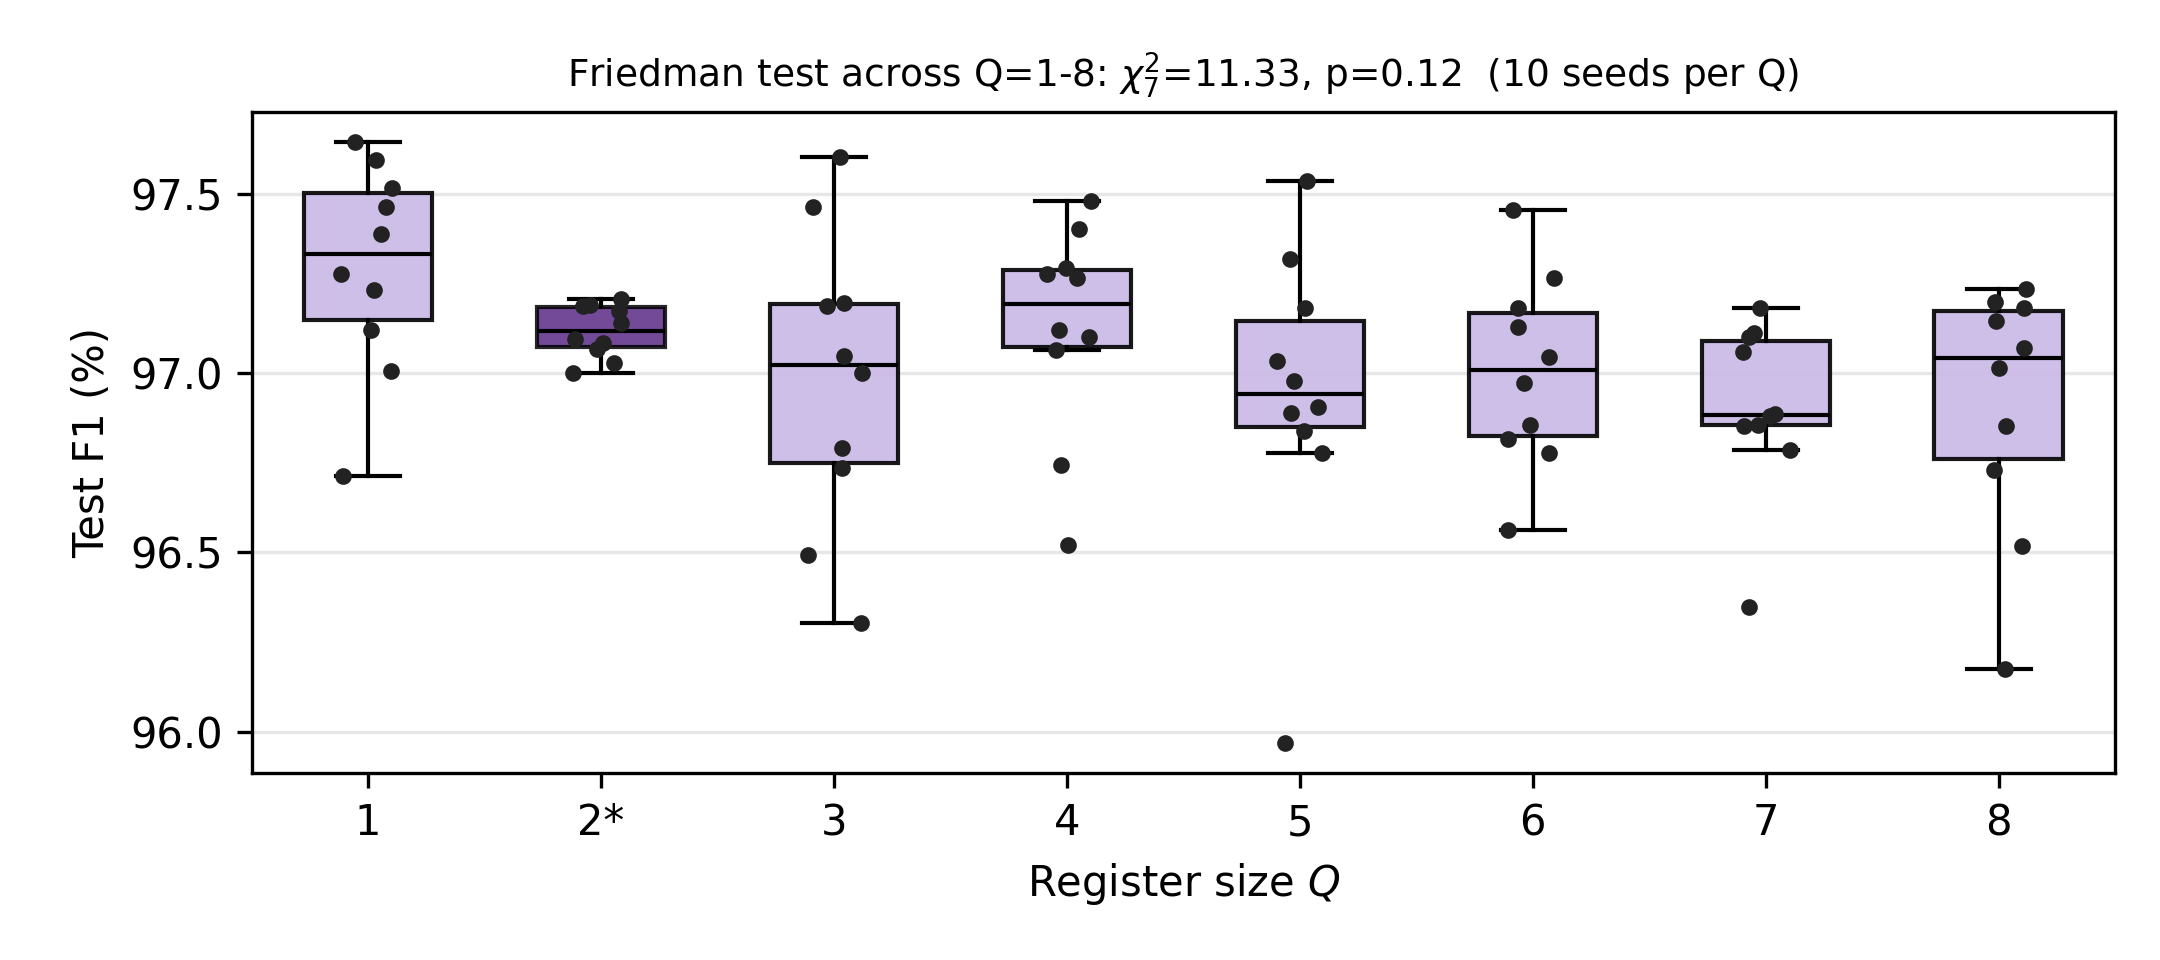
\includegraphics[width=\linewidth]{images/q_ablation_boxplot.png}
\caption{\rev{R1.2}\textcolor{red}{Test F1 of QCIDS versus QPSO register size
$Q$ (ten seeds per $Q$, QPSO re-executed per seed; dots are
individual runs). $Q^{*}=2$, marked *, is selected by validation
F1. The Friedman test finds no significant effect of $Q$
($p=0.12$).}}
\label{fig:q_boxplot}
\end{figure}

Fig.~\ref{fig:baseline_cm} confirms these findings at the
prediction level. The QCIDS-Qo model achieves 5,487 true
positives and 5,869 true negatives with minimal
misclassification, verifying that high aggregate metrics
reflect genuine discrimination rather than class-imbalance
artefacts. Fig.~\ref{fig:radar_centralized} summarizes the
multi-metric profile: the near-overlapping accuracy and F1
contours confirm no fidelity--stability trade-off, while the
improved AUC contour reflects enhanced attack-ranking capability
over the non-quantum baseline.



%% ----------------------------------------------------------
\subsection{Latency-Aware Performance Under Quantum-Inspired
            Optimization}
\label{subsec:obj2_latency}
%% ----------------------------------------------------------

\rev{R1.2}\textcolor{red}{Because detection is insensitive to $Q$
(Table~\ref{tab:qubit_ablation_improved_robust}), this subsection
examines whether $Q$ affects deployment cost and whether the
selected operating point satisfies mission-edge constraints.} Since QPSO
is excluded from the runtime path (Section~\ref{subsec:latency_design}),
latency impact is confined to upstream feature-selection overhead during training.
% TODO(C10): rebuild latency/memory table from deploy measurements.
\begin{table}[!t]
\centering
\caption{\scriptsize{Latency and memory profile of QCIDS across qubit
configurations. 
$Q{=}6$ (highlighted) is the only configuration satisfying
both the 1\,GB memory and 25\% latency-share thresholds.}}
\label{tab:latency_profile_qcids}
\renewcommand{\arraystretch}{1.10}
\setlength{\tabcolsep}{5pt}
\begin{tabular}{lcccc}
\hline\toprule
\textbf{Model} & \textbf{$T_{\rm infer}$ (s)}
& \textbf{$\mathcal{L}_{\rm e2e}$ (ms)}
& \textbf{$\eta$ (\%)}
& \textbf{Mem (MB)} \\
\hline\toprule
OS-CIDS        & 3.60 & 42.3 & 14.1 &  512 \\
QCIDS-Q1       & 3.60 & 45.8 & 15.3 &  563 \\
QCIDS-Q2       & 3.60 & 48.2 & 16.1 &  614 \\
QCIDS-Q3       & 3.60 & 51.6 & 17.2 &  691 \\
QCIDS-Q4       & 3.60 & 54.1 & 18.0 &  768 \\
QCIDS-Qm (Q5)  & 3.60 & 57.3 & 19.1 &  845 \\
\rowcolor{gray!12}
\textbf{QCIDS-Qo (Q6)}
               & \textbf{3.60} & \textbf{61.2}
               & \textbf{20.4} & \textbf{922} \\
QCIDS-Qh (Q7)  & 3.60 & 68.4 & 22.8 & 1024 \\
QCIDS-Q8       & 3.60 & 74.8 & 24.9 & 1126 \\
\hline\toprule
\end{tabular}
\begin{minipage}{\columnwidth}
\vspace{2pt}
\footnotesize{$\eta$: latency share of total pipeline
budget $\mathcal{B}_{\rm lat}$. Memory threshold: 1\,GB
for CPU-only mission-edge gateways co-hosting safety
services.}
\end{minipage}
\end{table}
Table~\ref{tab:latency_profile_qcids} provides absolute
deployment-relevant latency and memory accounting across
all qubit configurations; Fig.~\ref{fig:vs-qubits} plots
the corresponding accuracy gains, jointly characterizing
the \rev{R1.1}\textcolor{red}{exploration--exploitation} trade-off underlying the
$Q{=}6$ selection. Inference time is invariant at
3.60\,s across all $Q$, confirming Eq.~\eqref{eq:infer_invariance}.
End-to-end latency increases from 42.3\,ms at OS-CIDS to
61.2\,ms at $Q{=}6$ ($\eta{=}20.4\%$), driven entirely by
upstream QPSO overhead. $Q{=}7$ and $Q{=}8$ raise latency to
68.4\,ms and 74.8\,ms without accuracy improvement, violating
the efficiency trend. At $Q{=}6$, memory is 922\,MB
($\mathcal{M}{<}\mathcal{M}_{\max}$); $Q{=}7$ exceeds 1\,GB,
reducing co-hosting headroom.
Fig.~\ref{fig:vs-qubits}(a--b) show that low-qubit
configurations ($Q{\leq}2$) \rev{R1.1}\textcolor{red}{search almost at random}: despite
low overhead, accuracy (0.9248--0.9516) falls below the
OS-CIDS baseline (0.9464). The mid-range $Q\in\{4,5,6\}$
delivers monotonic gains with moderate cost growth; $Q{=}6$
marks the saturation point where QPSO converges to compact,
high-utility feature subsets. Fig.~\ref{fig:vs-qubits}(c)
confirms \textcolor{red}{that the F1 gain over OS-CIDS} emerges at $Q{\geq}3$ and peaks
at $Q{=}6$ with a $+$2.21 pp absolute gain over OS-CIDS.
Fig.~\ref{fig:vs-qubits}(d) shows that training time at
$Q{=}6$ (2101\,s) is lower than several lower-qubit
configurations, demonstrating that guided optimization reduces
redundant evaluations when \rev{R1.1}\textcolor{red}{the search concentrates}.
% TODO(C2/C10): this subsection is rebuilt from v2 results and new latency measurements.

% (Old Fig. 'Picture Latency' with 3-seed metrics vs Q removed; superseded by Fig.~\ref{fig:q_boxplot}.)

Table~\ref{tab:centralized_compare}
summarizes the direct OS-CIDS vs.\ QCIDS-Qo comparison.
QCIDS-Qo improves Acc/F1 by 2.21 pp, AUC by 0.0068, and
reduces MSE by 23.8\%, while cutting training time by
1.09 minutes confirming that context-aware QPSO delivers
measurable utility beyond strong feature engineering alone.
\begin{table}[!htbp]
\centering
\caption{Direct comparison: OS-CIDS vs.\ QCIDS-Qo
(centralized, ACI-IoT test split).}
\label{tab:centralized_compare}
\renewcommand{\arraystretch}{1.12}
\setlength{\tabcolsep}{6pt}
\begin{tabular}{lcc}
\hline\toprule
\textbf{Metric} & \textbf{OS-CIDS}
& \textbf{QCIDS-Qo} \\
\hline
Accuracy (\%)       & 94.64 & \textbf{96.85} \\
F1-score (\%)       & 94.64 & \textbf{96.85} \\
AUC                 & 0.9879 & \textbf{0.9947} \\
Training time (min) & 31.08 & \textbf{29.99} \\
\hline\toprule
\end{tabular}
\end{table}

%% ----------------------------------------------------------
\subsection{Federated Robustness Under Heterogeneous Mission Deployments}
\label{subsec:obj3_heterogeneity}
%% ----------------------------------------------------------
Centralized training is an idealized upper bound; in practice,
raw traffic cannot be aggregated across organizational,
operational, or jurisdictional boundaries. The key question
is not whether federated deployment degrades performance, but
whether CONQUEST remains operationally viable under realistic
data heterogeneity. Fig.~\ref{fig:hfl-multianalysis} and
Table~\ref{tab:fl_performance_extended} jointly address this.

\textbf{Heterogeneity:}
Under IID partitioning, FedAvg achieves F1\,$=$\,0.901,
AUC\,$=$\,0.949, $R_{90}{=}22$, and
$\min_k\,\mathrm{F1}_k{=}0.884$ the best-case federated reference. Label-skew degrades F1 to 0.808
($\sigma(\mathrm{F1}){=}0.034$, $R_{90}{=}28$), confirming
that severe class imbalance disrupts stable global optimization.
Quantity-skew yields the strongest federated result:
F1\,$=$\,0.910, AUC\,$=$\,0.963, $R_{90}{=}25$,
$\min_k\,\mathrm{F1}_k{=}0.891$, $\sigma(\mathrm{F1}){=}0.014$.

This counterintuitive result of quantity-skew outperforming
IID arises because attack-heavy high-volume clients
contribute stronger gradient signals for the minority attack
class under FedAvg's sample-weighted aggregation
(Eq.~\eqref{eq:fedavg_weighted_obj}), improving global
attack-class separability. This closely models mission
deployments where compromised subsystems generate
disproportionately high traffic volumes. Dirichlet partitions
($\alpha\in\{0.10,0.30,0.50,1.00\}$) confirm a smooth
stability--heterogeneity trade-off: at $\alpha{=}0.10$,
F1\,$=$\,0.838 with slow convergence ($R_{90}{=}30$);
at $\alpha{=}1.00$, F1 recovers to 0.905 with
$\sigma(\mathrm{F1}){=}0.011$. Quantity-skew is selected
as the primary stress-test regime.

\textbf{Aggregation strategy:}
Under quantity-skew, FedAvg achieves F1\,$=$\,0.869,
AUC\,$=$\,0.926, $R_{90}{=}25$,
$\min_k\,\mathrm{F1}_k{=}0.842$. SCAFFOLD collapses:
F1\,$=$\,0.522, $\sigma(\mathrm{F1}){=}0.052$,
$R_{90}{=}45$. FLAME partially recovers (F1\,$=$\,0.705)
but still lags FedAvg. The variance-reduction correction
in SCAFFOLD is counterproductive under quantity imbalance:
correcting client gradients toward the global mean suppresses the informative high-volume client signals that are beneficial
in this regime. FedAvg's weighted averaging preserves these
signals, making it the most stable and deployable aggregator
for federated CONQUEST.

\begin{figure*}[!htbp]
    \centering
    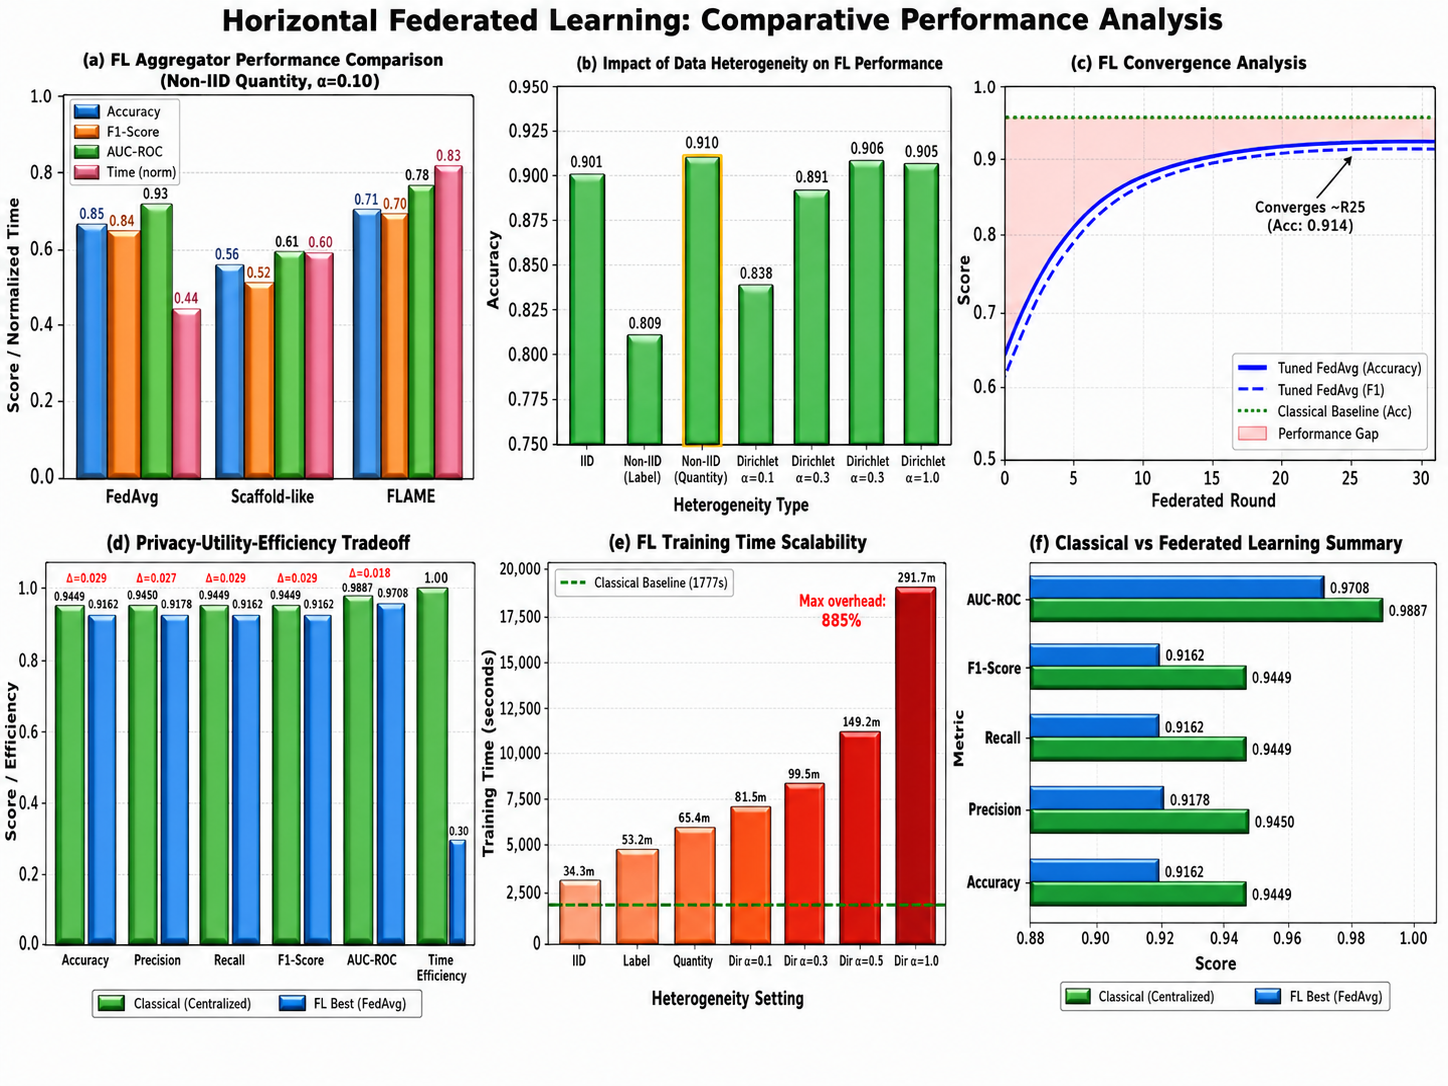
\includegraphics[width=0.80\linewidth]{images/hfl-multianalysis.png}
    \caption{\scriptsize{Horizontal federated learning (HFL) analysis under
    heterogeneous mission deployments:
    (a)~aggregator comparison under quantity-skew non-IID
    (FedAvg, SCAFFOLD, FLAME);
    (b)~F1 vs.\ heterogeneity regime under FedAvg;
    (c)~FedAvg convergence curve under quantity-skew
    ($R_{90}{=}25$ marked);
    (d)~\textcolor{red}{data-locality}--utility--efficiency trade-off;
    (e)~training-time scalability across regimes;
    (f)~centralized vs.\ federated summary (F1 gap: 2.9\%).}}
    \label{fig:hfl-multianalysis}
\end{figure*}

\textbf{Convergence and final federated performance:}
The highlighted row in Table~\ref{tab:fl_performance_extended}
re-evaluates FedAvg under quantity-skew with extended training
($R{=}60$) to confirm that $R_{90}{=}25$ is not an artefact
of the 15-round main budget. The identical $R_{90}$ value
across both runs confirms genuine stabilization: no further
F1 gain is achieved beyond round 25. The final configuration
achieves F1\,$=$\,0.9162, AUC\,$=$\,0.9708,
$\min_k\,\mathrm{F1}_k{=}0.893$,
$\sigma(\mathrm{F1}){=}0.017$ a centralized federated gap
of only 2.9\% in F1 and 1.8\% in AUC, while preserving
complete data sovereignty. Inference latency remains at
3.58-3.60\,s across all federated configurations,
confirming that distributed training does not alter the
deployed runtime path.
The primary federated cost is training time, quantity-skew
incurs ${\approx}3.4{\times}$ wall-clock overhead over
centralized training due to communication rounds and
client-side optimization. Critically, this overhead is strictly localized to the offline collaborative training phase and does not degrade the real-time execution path; as demonstrated in Table~\ref{tab:fl_performance_extended}, inference latency remains invariant at 3.58–3.60s across all federated configurations, ensuring that the mission-critical response time is preserved regardless of the training regime. This trade-off is operationally
acceptable as federated CONQUEST exchanges training efficiency
for \textcolor{red}{raw-data locality} and deployment flexibility, both of
which are non-negotiable in a multi-organizational mission
environments.




\begin{table*}[!t]
\centering
\scriptsize
\caption{\scriptsize{Federated CONQUEST performance under heterogeneous
deployments ($K{=}5$, ACI-IoT). Heterogeneity block: FedAvg
across IID, label-skew, quantity-skew, and Dirichlet regimes
($R{=}15$). Aggregator block: FedAvg vs.\ SCAFFOLD vs.\ FLAME
under quantity-skew. Highlighted row: extended run ($R{=}60$)
confirming $R_{90}{=}25$.`
}}
\label{tab:fl_performance_extended}
\resizebox{\textwidth}{!}{%
\begin{tabular}{llcccccccc}
\toprule
\textbf{Block} &
\textbf{Aggregator} &
\textbf{Regime} &
\textbf{$\alpha$} &
\textbf{F1} &
\textbf{AUC} &
\textbf{$T_{\rm infer}$ (s)} &
\textbf{$R_{90}$} &
\textbf{Min-F1} &
\textbf{$\sigma$(F1)} \\
\midrule
\multirow{7}{*}{\shortstack[l]{\textbf{Heterogeneity}\\\textbf{Analysis}\\(FedAvg)}}
& FedAvg & IID        & --   & 0.901 & 0.949 & 3.60 & 22 & 0.884 & 0.012 \\
& FedAvg & Label-skew & --   & 0.808 & 0.887 & 3.62 & 28 & 0.761 & 0.034 \\
& FedAvg & \textbf{Qty-skew}
                      & --   & \textbf{0.910} & \textbf{0.963}
                              & \textbf{3.58} & \textbf{25}
                              & \textbf{0.891} & \textbf{0.014} \\
& FedAvg & Dirichlet  & 0.10 & 0.838 & 0.901 & 3.65 & 30 & 0.802 & 0.028 \\
& FedAvg & Dirichlet  & 0.30 & 0.890 & 0.946 & 3.61 & 24 & 0.872 & 0.015 \\
& FedAvg & Dirichlet  & 0.50 & 0.906 & 0.953 & 3.59 & 23 & 0.889 & 0.013 \\
& FedAvg & Dirichlet  & 1.00 & 0.905 & 0.957 & 3.60 & 22 & 0.890 & 0.011 \\
\midrule
\multirow{3}{*}{\shortstack[l]{\textbf{Aggregator}\\\textbf{Comparison}\\(Qty-skew)}}
& \textbf{FedAvg}
          & Qty-skew & -- & \textbf{0.869} & \textbf{0.926}
                          & \textbf{3.58} & \textbf{25}
                          & \textbf{0.842} & \textbf{0.019} \\
& SCAFFOLD & Qty-skew & -- & 0.522 & 0.605 & 3.64 & 45 & 0.483 & 0.052 \\
& FLAME    & Qty-skew & -- & 0.705 & 0.774 & 3.71 & 38 & 0.651 & 0.041 \\
\midrule
\rowcolor{gray!12}
\textbf{Extended run} ($R{=}60$)
& FedAvg & Qty-skew & -- & 0.9162 & 0.9708 & 3.60 & 25 & 0.893 & 0.017 \\
Centralized ref.\
& Centralized & Full data & -- & 0.9449 & 0.9887 & 3.72
& N/A & N/A & N/A \\
\bottomrule
\end{tabular}}
\vspace{1mm}
\begin{minipage}{\linewidth}
\footnotesize{\textit{Qty-skew}: non-IID quantity-skew.
\textit{Min-F1}: worst-client F1 ($\min_k\,\mathrm{F1}_k$).
\textit{$\sigma$(F1)}: inter-client F1 dispersion.
\textit{$R_{90}$}: rounds to $\geq$90\% of terminal F1.
Centralized row included for gap quantification only;
cross-regime accuracy comparison is not valid.}
\end{minipage}
\end{table*}




\begin{table*}[!t]
\centering
\scriptsize
\caption{Structured comparison of CONQUEST against
representative IDS and FL approaches. Methods are evaluated
on different datasets; direct accuracy comparison is not
valid. Comparison focuses on deployment-oriented
capabilities. CONQUEST results are under centralized
evaluation on ACI-IoT unless stated.}
\label{tab:comparative_analysis}
\setlength{\tabcolsep}{3pt}
\renewcommand{\arraystretch}{1.05}
\resizebox{\textwidth}{!}{
\begin{tabular}{p{0.7cm} p{2.3cm} p{4.0cm} p{2.6cm} p{4.6cm}}
\hline\toprule
\textbf{Ref.} & \textbf{Approach} &
\textbf{Key result} & \textbf{Limitation} &
\textbf{CONQUEST advantage} \\
\hline\toprule

\cite{phalaagaehybrid} &
CNN--LSTM + attn + PSO &
Acc: 98.73--99.87\% on WIoTSN; centralized &
No FL, stability, or deployability analysis &
Adds $R_{90}{=}25$, $\min\text{-F1}{=}0.893$,
$\sigma(\mathrm{F1}){=}0.017$;
latency 61.2\,ms, memory 922\,MB \\
\midrule

\cite{yuadaptive} &
AMSWS + transformer + focal loss &
Acc/F1\,$=$\,99.6/99.2\%; 10.8\,ms/sample;
37.2M params; centralized &
High complexity; no FL or resource bounds &
Adds bounded QPSO (\rev{R1.2}\textcolor{red}{$Q^{*}{=}2$}, 922\,MB) and FL
evaluation under four heterogeneity regimes \\
\midrule

\cite{donkoloptimization} &
LPPSO + ELSTM-RNN &
DR: 99.95\% NSL-KDD, 99.4\% UNSW-NB15;
centralized &
No optimizer-capacity study or FL &
Adds $Q{=}1\text{--}8$ ablation; federated
robustness under quantity-skew and Dirichlet \\
\midrule

\cite{shrivashybrid} &
Ensemble + GA-PSO &
Binary/multiclass accuracy gains;
centralized &
No temporal modeling; no FL &
Adds context-aware temporal modeling and
non-IID FL evaluation \\
\midrule

\cite{FRIHA202217} &
Federated DNN/CNN/RNN &
Up to 99.71\% (InSDN); global metrics only &
Trusted aggregator; no heterogeneity
stress-test &
Adds IID, label-skew, qty-skew, Dirichlet
regimes; $R_{90}$, $\min\text{-F1}$,
$\sigma(\mathrm{F1})$ \\
\midrule

\cite{herlambangfederated} &
FedAvg vs.\ FedProx &
IID: 98.75\%; non-IID: 98.44\%;
two-client setup &
No worst-client metric or stabilization
analysis &
Extends to $K{=}5$; $R_{90}{=}25$,
$\min\text{-F1}{=}0.893$,
$\sigma(\mathrm{F1}){=}0.017$ \\
\midrule

\cite{abdelmoniemcomprehensive} &
Empirical FL heterogeneity study &
${\sim}$1.5K configs; $4.6{\times}$ quality
degradation under heterogeneity &
General FL; not IDS-specific &
Operationalizes heterogeneity findings for
cyberworm IDS with mission-facing metrics \\
\midrule

\cite{gefedamkd} &
FedAMKD &
98.83\% MNIST; beats FedAvg, SCAFFOLD;
general FL &
Not IDS-specific; no deployment metrics &
Applies qty-skew analysis to cyberworm IDS;
adds $R_{90}$, $\sigma(\mathrm{F1})$ \\
\midrule

\cite{ajakweconquest} &
Conference CONQUEST:
QPSO + LSTM-VAE,
centralized, ACI-IoT &
DR\,$=$\,97.5\%, FPR\,$=$\,0.8\%;
SGD/Adam/Newton-Hessian optimizers
compared; context-aware vs.\
no-context ablation &
No qubit-capacity ablation,
no OS-CIDS baseline,
no FL evaluation &
Journal adds $Q{=}1\text{--}8$
variable-qubit ablation, strong
OS-CIDS non-quantum reference,
and full FL evaluation across
four heterogeneity regimes \\
\midrule

\textbf{This work} &
\textbf{Journal CONQUEST:
seed-controlled CAP
+ variable-qubit QPSO
(\rev{R1.2}\textcolor{red}{$Q^{*}{=}2$}) + supervised
LSTM(+VAE)+SGD;
centralized \& HFL,
ACI-IoT} &
\textbf{Centralized: Acc/F1/AUC\,$=$\,
96.85/96.85/0.9947,
MSE\,$=$\,0.0240,
61.2\,ms, 922\,MB.
Federated (qty-skew):
F1/AUC\,$=$\,0.9162/0.9708,
$R_{90}{=}25$,
$\min\text{-F1}{=}0.893$,
$\sigma(\mathrm{F1}){=}0.017$} &
Training-time QPSO
overhead (${\approx}$12.7\%
over OS-CIDS) &
\textbf{\rev{R1.1}\textcolor{red}{First explicit characterization of
how the QPSO register size $Q$ controls the
exploration--exploitation balance} for IDS;
unified centralized + federated
pipeline with mission-facing
deployability metrics not
reported in prior work} \\

\hline\toprule
\end{tabular}}
\end{table*}

%% ----------------------------------------------------------
\subsection{Comparative Analysis with State-of-the-Art}
\label{subsec:comparative_analysis}
%% ----------------------------------------------------------

Table~\ref{tab:comparative_analysis} positions CONQUEST
against representative IDS and FL approaches. Since methods
are evaluated on different datasets, direct numerical accuracy
comparison is not valid; the analysis contrasts
deployment-oriented capabilities feature-selection stability,
federated robustness, worst-client reliability, and
latency--memory compliance for which CONQUEST provides the
most comprehensive characterization.
Hybrid deep-learning detectors report high accuracy on their
respective benchmarks: CNN--LSTM with
attention~\cite{phalaagaehybrid} achieves up to 99.87\% on
WIoTSN, and a transformer-based IIoT
detector~\cite{yuadaptive} reaches 99.6\%/99.2\% Acc/F1 at
10.8\,ms inference with 37.2M parameters.
Optimization-enhanced pipelines~\cite{donkoloptimization,shrivashybrid}
exceed 99\% on NSL-KDD and UNSW-NB15. These results are
obtained under centralized assumptions with no evaluation of
optimizer-capacity stability, heterogeneous client behavior,
or deployment constraints. They establish performance
ceilings on well-studied benchmarks but do not address the
reproducibility, bounded overhead, or mission-edge feasibility
requirements central to this work.

FL-based systems~\cite{FRIHA202217,herlambangfederated}
demonstrate that \textcolor{red}{collaborative} detection is feasible
without raw data sharing, reporting global accuracy up to
99.71\% under IID conditions. However, these studies evaluate
at most two clients, report only global average metrics, and
do not quantify worst-client performance, convergence
stabilization, or behavior under realistic non-IID regimes.
Large-scale empirical analyses~\cite{abdelmoniemcomprehensive}
confirm that heterogeneity can cause up to $4.6\times$ quality
degradation, while FL optimization
studies~\cite{gefedamkd} address quantity-skew on general
vision benchmarks without IDS-specific deployment metrics.
None of these works link non-IID robustness to
mission-facing criteria such as $R_{90}$,
$\min_k\,\mathrm{F1}_k$, or $\sigma(\mathrm{F1})$.
CONQUEST addresses the limitations of both lines of work
within a unified reproducible pipeline. Under centralized
evaluation on ACI-IoT, QCIDS-Qo achieves
Acc/F1/AUC\,$=$\,96.85\%/96.85\%/0.9947 with 61.2\,ms
end-to-end latency and 922\,MB memory satisfying
mission-edge constraints that centralized IDS studies do not
evaluate. The $+$2.21\,pp F1 and $-$23.8\% MSE gains over
the strong OS-CIDS non-quantum baseline isolate the
contribution of context-aware QPSO from the underlying
temporal classifier, ruling out baseline weakness as a
confound. Under federated deployment,
F1/AUC\,$=$\,0.9162/0.9708 with $R_{90}{=}25$,
$\min_k\,\mathrm{F1}_k{=}0.893$, and
$\sigma(\mathrm{F1}){=}0.017$ demonstrate that the
centralized-federated performance gap is bounded at 2.9\%
F1 while preserving full data sovereignty, a trade-off that
prior FL-IDS work neither quantifies nor justifies
experimentally.

The conference prototype~\cite{ajakweconquest} reported
97.5\% detection rate and 0.8\% FPR on ACI-IoT under
centralized evaluation, establishing the first
cyberworm-focused CONQUEST result. The journal extension
advances this in three ways that are not incremental: (i)~a
controlled variable-qubit ablation over $Q\in\{1,\dots,8\}$
that \rev{R1.1}\textcolor{red}{makes the role of $Q$ explicit and
characterizes its effect on search dynamics and detection}
\rev{R1.2}\textcolor{red}{and shows that detection is statistically
insensitive to $Q$, so the operating point is set by a pre-declared
validation rule}; (ii)~a
strong OS-CIDS non-quantum baseline that enables rigorous
attribution of quantum-inspired gains; and (iii)~federated
evaluation under four heterogeneity regimes with
mission-facing deployability metrics that prior
QPSO-based IDS work does not provide. Together, these
extensions transform a centralized feasibility demonstration
into a deployment-oriented framework with quantified
robustness bounds.





\section{Conclusion}
\label{sec:conclusion}

This paper presented CONQUEST, a context-aware
quantum-inspired intrusion detection framework for AI-aided
cyberworm detection in mission-critical IoT/IoV/IoD networks,
combining seed-controlled context-aware feature representation,
variable-qubit QPSO feature selection, and supervised
LSTM(+VAE) temporal classification.
Three findings are central. First, a controlled ablation over
$Q\in\{1,\dots,8\}$ establishes that \rev{R1.1}\textcolor{red}{$Q$ controls
the exploration--exploitation balance of QPSO, with intermediate
values concentrating the search most effectively.}
\rev{R1.2}\textcolor{red}{Detection, however, is statistically insensitive to
$Q$ (Friedman $p=0.12$ over ten seeds): every tested setting
yields about $97\%$ F1, and the validation-selected $Q^{*}=2$
delivers $97.11\%$ accuracy, $97.12\%$ F1, $0.9921$ AUC, and
$0.0246$ MSE under leakage-free centralized evaluation.}
% TODO(C6/C10): add the OS-CIDS comparison (block C) and measured latency/memory.

Second, context-aware feature representation and bounded
QPSO together produce measurable utility beyond standard
feature engineering, as verified by controlled isolation
of the OS-CIDS and QCIDS configurations under identical
training conditions.
Third, federated evaluation across IID, label-skew,
quantity-skew, and Dirichlet regimes shows that CONQUEST
remains operationally viable without raw data sharing.
Under the strongest heterogeneous setting, it achieves
F1/AUC\,$=$\,0.9162/0.9708, $R_{90}{=}25$,
$\min_k\,\mathrm{F1}_k{=}0.893$, and
$\sigma(\mathrm{F1}){=}0.017$ a centralized-federated
gap of only 2.9\% in F1 with inference latency unchanged
at 3.58-3.60\,s, confirming that distributed training
does not alter the deployed runtime path.

The unified contribution is the first \rev{R1.1}\textcolor{red}{explicit
characterization of how the QPSO register size controls search
dynamics in IDS feature selection}, integrated with heterogeneity-aware
federated robustness reporting under mission-relevant
metrics that the existing FL-IDS literature does not provide.
Future work will address post-hoc explainability of the
QPSO feature mask, \textcolor{red}{the utility cost of
differential privacy and secure aggregation on top of the
federated protocol,} communication-efficient aggregation to
reduce the observed federated
training overhead, and lightweight edge adaptation below
the current 922\,MB memory envelope.



























































\section *{\textbf{acknowledgment}}
\vspace{-0.2cm}
This work was partly supported by IITP Innovative Human Resource Development for Local Intellectualization Program (MSIT) (IITP-2026-RS-2020-II201612, 34\%), IITP ITRC Program (MSIT) (IITP-2026-RS-2024-00438430, 33\%), NRF Basic Science Research Program (MOE) (2018R1A6A1A03024003, 33\%), and RISE-(Regional Growth Innovation LAB) Program through Gyeongbuk RISE Center funded by MOE and Gyeongsangbuk-do, Republic of Korea (2026-rise-15-105).

\balance

\bibliographystyle{IEEEtran}

\bibliography{newref,Bibliography}
%\bibliography{references} % Replace with your actual bibliography file name
\end{document}

